%------------------------------------------------------------
% PACOTES E CONFIGURAÇÃO DO TEMPLATE

\documentclass[12pt]{article}
\usepackage[utf8]{inputenc} % Acentos
\usepackage[brazil]{babel}  % Nomes em português
\usepackage[utf8]{inputenc}
\usepackage{natbib}
\usepackage{graphicx}
\usepackage[T1]{fontenc}
\usepackage{authblk}
\usepackage{color}
\usepackage{setspace}
\usepackage{tabularx}
\usepackage{longtable}
\usepackage{titlesec}
\usepackage{hyperref}
\usepackage{float}
\usepackage{scrextend} 
\usepackage{longtable}
\usepackage{indentfirst}
\usepackage{array}
\usepackage{geometry}
\usepackage{fancyhdr}
\usepackage{algorithmic}
\usepackage[portuguese, ruled, linesnumbered]{algorithm2e}
\usepackage[nottoc,notlot,notlof]{tocbibind}
\usepackage[titletoc]{appendix}

%margens
\geometry
{
    a4paper,
    left=20mm,
    top=30mm,
    right=20mm,
    bottom=20mm
}

\pagestyle{fancy} %Ativa o estilo
\fancyhf{} %Começa limpando tudo no header and footer
\fancyfoot[R]{\thepage} %Númeração no lado inferior direito
\renewcommand{\headrulewidth}{0pt}%tira a linha do header
\newcommand{\tab}[1]{\hspace{.2\textwidth}\rlap{#1}}
\newcolumntype{C}[1]{>{\centering}p{#1}} % coluna
\newcommand{\daniel}[1]{\textcolor{blue}{#1}} %comentários de Daniel

%para a quebra de linhas dentro de uma célula na tabela
\newcommand{\specialcell}[2][c]{
  \begin{tabular}[#1]{@{}l@{}}#2\end{tabular}}
  
\renewcommand{\baselinestretch}{1.5} %espaçamento entre linhas
  
\graphicspath{ {figures/} }

%BLOCO DA FOLHA DE RESTO FICAR NA DIREITA
\def\changemargin#1#2{\list{}{\rightmargin#2\leftmargin#1}\item[]}
\let\endchangemargin=\endlist 

%PRA ADICIONAR SUBSUBSUBSECTION
\titleclass{\subsubsubsection}{straight}[\subsection]

\newcounter{subsubsubsection}[subsubsection]
\renewcommand\thesubsubsubsection{\thesubsubsection.\arabic{subsubsubsection}}

\titleformat{\subsubsubsection}
  {\normalfont\normalsize\bfseries}{\thesubsubsubsection}{1em}{}
\titlespacing*{\subsubsubsection}
{0pt}{3.25ex plus 1ex minus .2ex}{1.5ex plus .2ex}
\makeatletter
\def\toclevel@subsubsubsection{4}
\def\l@subsubsubsection{\@dottedtocline{4}{7em}{4em}}
\makeatother
\setcounter{secnumdepth}{4}
\setcounter{tocdepth}{4}

%------------------------------------------------------------
% INÍCIO DO DOCUMENTO
\begin{document}

    %------------------------------------
    % CAPA
    \begin{titlepage}
    \begin{center}
    
\includegraphics[width=3cm]{images/logoufpe.jpg}\\
    \large Universidade Federal de Pernambuco\\
    \large Centro de Informática - CIn
    \vskip1cm
    \large Graduação em Engenharia da Computação\\
    \vskip3cm
    
    {\textbf
        {\LARGE 
            Comparativo de Técnicas de Aprendizado de Máquina para o Treinamento de Grids Regulares na Técnica de Localização por Fingerprinting
        }
    }
    
    \vskip2cm

    \large Anderson Augusto Freitas Urbano\\
    \large TRABALHO DE GRADUAÇÃO\\
    \vskip2cm
    Recife, \today
    \vskip2cm
    
\includegraphics[width=5cm]{images/logo-cin.jpg}    
    \end{center}
    \end{titlepage}
    
    %------------------------------------
    % SEGUNDA CAPA
    \newpage
    \thispagestyle{empty}%esconder o número da página
    \begin{center}
    \large Universidade Federal de Pernambuco\\
    \large Centro de Informática - CIn
    \vskip1cm
    \large Graduação em Engenharia da Computação\\
    \vskip3cm  
   
    {\textbf
        {\LARGE 
            Comparativo de Técnicas de Aprendizado de Máquina para o Treinamento de Grids Regulares na Técnica de Localização por Fingerprinting
        }
    }

    \end{center}
    \vskip4cm
   
    \begin{addmargin}[10em]{0em}
    \large
    Trabalho apresentado ao Programa de Graduação em Engenharia da Computação do Centro de Informática da Universidade Federal de Pernambuco como requisito parcial para obtenção do grau de Bacharel em Engenharia da Computação.
    \end{addmargin}
   
    \vskip5cm
   
    \begin{flushleft}
    \large{\textbf{Aluno: }Anderson Augusto Freitas Urbano}\\
    \large{\textbf{Orientador: }Daniel Carvalho da Cunha}
    \end{flushleft}     
    
    %------------------------------------
    % AGRADECIMENTOS
    \newpage
    \thispagestyle{empty}
    \begin{center}
    \textbf{\LARGE Agradecimentos}
    \end{center}

    Agradeço a algumas pessoas que me ajudaram imensamente na tarefa de concluir este trabalho. Primeiramente aos meus pais, que sempre me deram apoio e incentivo em todos os momentos da minha vida. Agradeço também à minha irmã e a todos os meus familiares sem os quais não poderia ter chegado onde estou.
    
    A meus colegas e amigos do centro de informática que tantas vezes me auxiliaram em meu aprendizado e realização de meus projetos desde o início do curso, em especial, Gustavo, Diogo e Larissa que me ajudaram diretamente com este trabalho.
    
    A todos os meus professores das escolas e do centro de informática, incluindo especialmente, meu orientador Daniel da Cunha que mostrou-se um ótimo professor, sempre prestativo e de grande ajuda tanto na produção deste trabalho científico quanto em todas as disciplinas que cursei com ele.
    
    E finalmente a todos os meus amigos, namorada e pessoas que se importam e estiveram comigo nos bons e maus momentos e para os quais tenho muito carinho e apreço.
    \vskip3mm
    Obrigado.

    %------------------------------------
    % RESUMO
    \newpage
    \thispagestyle{empty}
    \begin{center}
    \textbf{\LARGE Resumo}
    \end{center}

    \par{
    A localização \textit{outdoor} de dispositivos móveis já possui diversas aplicações e pode ser executada por algumas técnicas conhecidas na literatura. Entre elas está a técnica de \textit{fingerprinting} que embora não seja tão precisa quanto o Sistema de Posicionamento Global (GPS) pode alcançar precisões de algumas dezenas de metros e ser aplicada em ambientes urbanos utilizando as redes de telefonia móvel celular existentes demandando pouca ou nenhuma mudança na infraestrutura das mesmas. A técnica baseada em \textit{fingerprinting} divide a região geográfica de interesse em um GRID de células com informações de nível de sinal para as estações de serviço de telefonia móvel da região. Essa informação pode ser gerada a partir da coleta de medições de nível de sinal e técnicas de aprendizado de máquina. Este trabalho propõe fazer um comparativo e análise de desempenho de diferentes algoritmos de aprendizado de máquina aplicados no treinamento de GRIDs regulares, que possuem espaçamento igual entre suas células, utilizados para a localização \textit{outdoor} com \textit{fingerprinting}.  
    }
    
    \vspace{10pt}
    
    \par{\textbf{Palavras-chaves:} Localização Outdoor; Localização Baseada em Sinal; Fingerprinting; GRIDs Regulares; Aprendizado de Máquina; Redes Celulares.}

    %------------------------------------
    % ABSTRACT
    \newpage
    \thispagestyle{empty}
    \begin{center}
    \textbf{\LARGE Abstract}
    \end{center}
    
    \par{
    Outdoor location systems for mobile devices already has many different applications in literature. Among these techniques is the Fingerprinting method, which, although not as precise as the Global Positioning System (GPS), it can achieve tens of meters precision and be implemented with few or no modifications to the current cellular network infraestructure as a critical advantage. The \textit{fingerprinting} based technique using divides the geographic region in a GRID of cells with Received Signal Strengh Indicator (RSSI) information to the radio base station providing service to the region. This information can be generated from RSSI measurements and machine learning techniques. This work makes a comparative and performance analysis of different machine learning algorithms applied in training of regular GRIDs, which have regular space between cells, used for outdoor location with \textit{fingerprinting}. 
    }
    
    \vspace{10pt}
    
    \begin{sloppypar}
    \par{\textbf{Keywords:} Outdoor Positioning; Signal Based Positioning; Fingerprinting; Regular GRIDs; Machine Learning;  Cellphone Networks.}
    \end{sloppypar}
    
    %------------------------------------
    % LISTA DE FIGURAS
    \newpage
    \listoffigures
    
    %------------------------------------
    % LISTA DE TABELAS
    \newpage
    \listoftables

    %------------------------------------
    % SUMÁRIO
    \newpage
    \thispagestyle{empty}
    \tableofcontents

    %------------------------------------
    % INTRODUÇÃO
    \newpage
    \section{Introdução}
    \label{sec:introducao}
        
    Sistemas de localização já estão sendo utilizados nas mais diversas formas nos dias atuais (ver \cite{taxonomyLocationServices2003}), como navegação, planejamento de rotas, segurança e até jogos digitais e aplicações em redes sociais. Usuários podem ter acesso à sua informação de localização de maneira simples e prática através de \textit{smartphones} ou outros dispositivos móveis.
        
    Existem diversos sistemas de localização utilizando a infraestrutura de comunicação celular na literatura, como as baseadas em modelos de propagação de ondas de rádio e as tecnologias de GPS (\textit{Global Positioning System}) Assistido. Cada sistema possui suas características, vantagens e desvantagens em relação a outros. Em geral, é preciso considerar a precisão, custo e área de cobertura de um sistema a ser implementado (\cite{locationSystems2008}).
        
    Neste contexto a técnica de \textit{fingerprinting} para localização entra como uma técnica de precisão mediana porém de baixo custo e que pode ser incorporada facilmente às redes de telefonia celular existentes, se tornando um alternativa interessante para se agregar aos sistemas atuais.
        
    A técnica baseada em \textit{fingerprinting} divide a região geográfica de interesse em subregiões e atua de maneira a mapear o nível de sinal das estações rádio base (ERBs) provedoras de serviço de telefonia em cada subregião, formando assim um mapa de identificadores únicos para cada subregião conhecidos como \textit{fingerprints} ou impressões digitais. A partir desse mapa é possível estimar a posição mais provável do móvel comparando a sua impressão digital com as impressões mapeadas.
        
    O mapa do \textit{fingerprinting} consiste de um GRID de células que pode ser regular ou irregular, isto é, possui células iguais e igualmente espaçadas ou não e o treinamento desse GRID pode ser feito utilizando algoritmos de aprendizado de máquina para regressão de maneira a estimar o nível de sinal em cada ponto do mapa baseado em amostras pré-existentes.
        
    Neste trabalho foram avaliados 4 algoritmos diferentes de regressão para treinamento de um GRID regular de células: K Vizinhos Mais Próximos (\textit{K Nearest Neighbors}, KNN), \textit{Perceptron} Multicamadas (\textit{Multilayer Perceptron}, MLP), Máquina de Vetores de Suporte (\textit{Support Vector Machine}, SVM) e \textit{Random Forest}. Além disso, é realizada uma análise comparativa das técnicas adotadas com base em métricas de erro.
    
        %------------------------------------
        % OBJETIVOS
        \subsection{Objetivos}
        \label{sec:objetivos}
    
        Este trabalho tem por objetivos:
        
        \begin{enumerate}
            \item Implementar a técnica de \textit{fingerprinting} utilizando um GRID regular de células;
            
            \item Analisar eficácia de 4 diferentes algoritmos de aprendizado de máquina para treinamento do GRID regular aplicado na tarefa de localização.
        \end{enumerate}
    
        %------------------------------------
        % ESTRUTURA DO DOCUMENTO
        \subsection{Estrutura do Documento}
        \label{sec:estruturaDocumento}
    
        O trabalho está estruturado de maneira que o Capítulo \ref{sec:conceitosBasicos} terá uma revisão de conceitos básicos sobre localização \textit{outdoor}, \textit{fingerprinting} e algoritmos de aprendizado de máquina para regressão. O Capítulo \ref{sec:metodologia} mostra a metodologia experimental planejada e os principais resultados obtidos. Por fim o Capítulo \ref{seq:conclusao} trará conclusões gerais e trabalhos futuros. As tabelas completas de resultados obtidos para todos os experimentos estão contidas no Apêndice \ref{appendix:fulltables}.

    %------------------------------------
    % CONCEITOS BÁSICOS
    \newpage
    \section{Conceitos Básicos}
    \label{sec:conceitosBasicos}

        %------------------------------------
        % LOCALIZAÇÃO EM SISTEMAS DE TORRES DE CELULAR
        \subsection{Localização em Sistemas de Telefonia Celular}
        \label{sec:localizacao}
        
        Os sistemas de telefonia móvel celular, de maneira simplificada, constituem uma rede de comunicação sem fio que utiliza estações de rádio espalhadas por uma determinada região em que cada estação atende aos dispositivos móveis dentro de sua área de cobertura. O dispositivo comunica-se com a sua estação para efetuar chamadas telefônicas, acesso a dados e outras operações, incluindo determinar as suas coordenadas geográficas. 
        
        Segundo \cite{locationSystems2008}, as técnicas de localização utilizando a infraestrutura de telefonia móvel celular podem ser divididas em 4 categorias de técnicas principais:
        
        \begin{itemize}

        \item{\textbf{Baseadas em \textit{cell-ID}}}: É o método relativamente mais simples. Utiliza a identificação (\textit{cell-ID}) da estação que está provendo serviço de telefonia ao móvel. Como a localização das estações é conhecida, então a localização do movél estará dentro da área de cobertura da sua estação atual. Esta área de cobertura pode variar de centenas de metros em áreas urbanas para algumas dezenas de quilômetros em áreas rurais portanto este método de localização não atende aos requisitos de localização de aplicações que exijam grande precisão na posição estimada porém requer pouco esforço de implementação pois não necessita de muitas informações.  
    
        \item{\textbf{Baseadas em modelos de propagação de ondas de rádio}}: Esse tipo de técnica estima a distância até as estações rádio base disponíveis em geral a partir da trilateração de distâncias do movél até essas estações (sendo necessárias no mínimo 3 estações). 
        
        As variações com nível de sinal estimam essa distância pela degradação do nível de sinal recebido pelo móvel em relação ao sinal enviado pela estação (conhecido previamente). Isso requer um modelo de propagação do sinal e estes, em geral, fazem suposições sobre as características do terreno e são muito menos precisos em ambientes urbanos.
        
        As variações por tempo de chegada (\textit{Time of Arrival}, ToA) e diferença de tempo de chegada (\textit{Time Difference of Arrival}, TDoA) utilizam informação de tempo em vez de nível de sinal. A primeira calcula a distância até cada estação rádio base a partir do tempo de voo (\textit{time-of-flight}) do sinal num processo conhecido como trilateração. Isso requer que tanto o móvel quanto as estações possuam relógios sincronizados, o que dificulta a implementação da técnica em alguns sistemas. O TDoA entretanto, sincroniza apenas as estações rádio base. É feito o \textit{broadcast} do sinal do móvel para cada estação e a diferença de tempo entre a chegada nas estações permite estimar a posição do móvel. Esta técnica, ao contrário da anterior, faz uma multilateração da posição e não uma trilateração.  
         
        É possível utilizar também o Ângulo de Chegada (\textit{Angle of Arrival}, AoA) do sinal a partir das estações rádio base. Isso requer uma infraestrutura com antenas direcionais. Baseado no ângulo de recebimento do sinal no móvel de pelo menos 2 estações estima-se a posição deste.
    
        \item{\textbf{As Tecnologias de GPS Assistido}}: A tecnologia de GPS funciona a partir da trilateração das distâncias do receptor a satélites orbitando a terra. Os receptores de GPS em geral necessitam de um espaço limpo para receber informações dos satélites, o que é um problema em ambientes urbanos, além de grande poder de processamento para calcular suas posições e determinar uma localização precisa do móvel, o que acarreta em maior consumo de bateria. O GPS Assistido ou AGPS (\textit{Assisted Global Positioning System}) utiliza a rede de telefonia móvel celular para fornecer informações dos satélites para o móvel conectado à rede, além disso parte do processamento pode ser feito pela rede, o que faz o móvel conseguir uma aquisição de localização mais rápida e com menos processamento necessário e portanto menor consumo de bateria.
        
        \item{\textbf{Estimativas Baseadas \textit{Fingerprinting} de Rádio}}: A categoria de técnicas a que este trabalho se dedica. Trata-se de técnicas empíricas que dividem uma área em regiões que podem ser identificadas unicamente por um conjunto de informações que formam uma impressão digital ou \textit{fingerprint}. Uma visão mais aprofundada do \textit{Fingerprinting} será apresentada na Seção \ref{sec:fingerprinting}. 
    
        \end{itemize}

        %------------------------------------
        % TÉCNICA DE FINGERPRINTING
        \subsection{Técnica de Localização por \textit{Fingerprinting}}
        \label{sec:fingerprinting}
    
        A técnica de localização por \textit{Fingerprinting} é bastante conhecida na literatura (vide \cite{surveyFingerprinting2016}). Consiste em uma abordagem empírica com duas etapas principais: a primeira forma uma base de dados de identificadores únicos associados a uma determinada localização a partir de um conjunto de informações coletadas nesta. A segunda etapa estima a posição do dispositivo móvel comparando o conjunto de informações atual do dispositivo com a base de dados e selecionando o local do identificador mais compatível com este conjunto (\textit{Matching}).

            %------------------------------------
            % ARQUITETURA DO FINGERPRINTING
            \subsubsection{Arquitetura Geral}
            \label{sec:arquiteturaFingerprinting}

            A arquitetura geral apresentada na Figura \ref{fig:arquiteturaGeralFingerprinting} é uma versão adaptada da apresentada em \cite{surveyFingerprinting2016}. Nela existe uma região a ser mapeada (uma cidade ou um bairro por exemplo) e é executada uma coleta de \textit{fingerprints} ou identificadores em pontos diferentes da região, guardando também as coordenadas de cada identificador. Isso irá formar uma base de dados para ser utilizada durante o processo de  \textit{matching} de novos \textit{fingerprints}.
            
            É importante notar que as informações que podem formar os \textit{fingerprints} podem ser de diversas naturezas. Em \cite{surveyFingerprinting2016}, é mostrado que os \textit{smartphones} atuais possuem uma vasta gama de sensores entre câmeras, microfones, acelerômetros, giroscópios além dos sensores para tecnologias de comunicação móvel via rádio. Todos esses sensores podem fornecer informações que em conjunto podem ser capazes de identificar uma localização, exemplos disso são imagens de \textit{landmarks}, som ambiente gravado, distâncias percorridas e é claro, nível de sinal de redes wifi e (o foco deste trabalho) de estações provedoras de serviço de sistemas de telefonia móvel celular.
            
            As informações obtidas durante a etapa de coleta muitas vezes necessitam de algum tipo de pré-processamento antes de gerar \textit{fingerprints}, como é o caso de encontrar descritores de imagens ou reduzir o ruído em outros sensores. Outro caso comum é utilizar várias medições coletadas no local para formar um identificador mais generalizado. Essa etapa é importante pois filtra informações desnecessárias e melhora a precisão do sistema, além reduzir o armazenamento necessário para a base de dados de \textit{fingerprints}.
            
            Um \textit{fingerprint} da base de dados seria então, como mostrado na Figura \ref{fig:fingerprintUnico}, um vetor de informações identificadoras em conjunto com as coordenadas do local que o \textit{fingerprint} identifica na região. É importante salientar que a construção da base de dados na maioria dos casos é executada de maneira \textit{offline} para reduzir os custos computacionais ao estimar a posição do móvel.
            
            Após a criação da base de \textit{fingerprints}, é possível estimar a localização de um dispositivo móvel gerando o seu \textit{fingerprint} a partir das informações atuais do dispositivo e encontrando o identificador mais compatível dentro da base de dados através de um algoritmo de \textit{matching}. Esse algoritmo irá possuir diferentes complexidades dependendo do tipo de dado a ser analisado e 
            pode empregar técnicas de aprendizado de máquina para encontrar as melhores combinações.
            
            \begin{figure}[H]
                \centering
                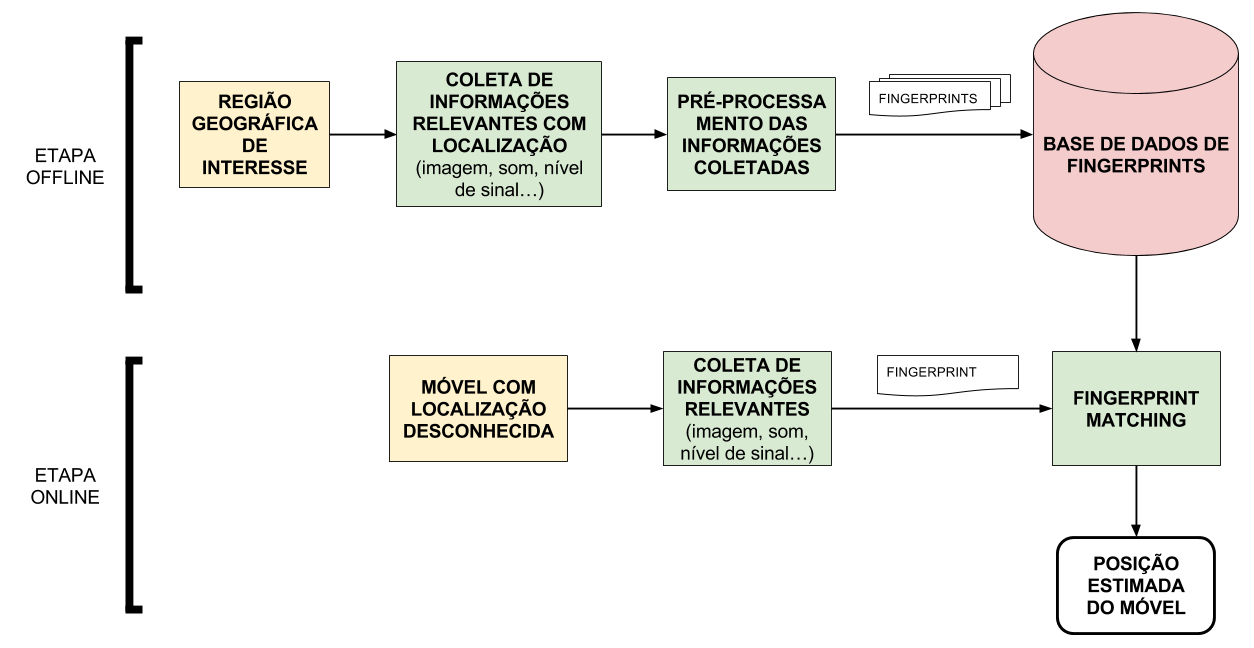
\includegraphics[width=16cm]{images/arquiteturaGeral.png}\par
                \caption{Arquitetura geral da técnica baseada em  \textit{Fingerprinting} (Adaptado de \cite{surveyFingerprinting2016}).}
                \label{fig:arquiteturaGeralFingerprinting}
            \end{figure}
            
            \begin{figure}[H]
                \centering
                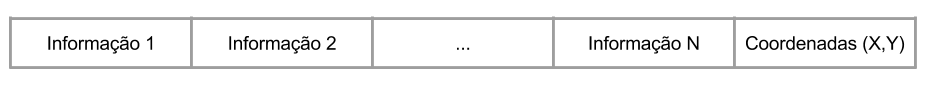
\includegraphics[width=14cm]{images/fingerprintUnico.png}\par
                \caption{Modelo geral de um \textit{Fingerprint}.}
                \label{fig:fingerprintUnico}
            \end{figure}
            
            %------------------------------------
            % ARQUITETURA DO FINGERPRINTING COM RSSI
            \subsubsection{\textit{Fingerprinting} utilizando nível de sinal}
            \label{sec:arquiteturaFingerprintingRSSI}
            
            A partir do modelo mostrado na Seção \ref{sec:arquiteturaFingerprinting} é possível gerar um modelo de \textit{Fingerprinting} que utilize o nível de sinal ou RSSI (\textit{Received Signal Strength Indicator}) sentido pelo dispositivo móvel das estações rádio base ou ERBs presentes no sistema de telefonia celular da região de interesse. O modelo apresentado na Figura \ref{fig:arquiteturaFingerprintingRSSI} ilustra as modificações necessárias no modelo geral e cada etapa será detalhada nas próximas Seções.
            
            Esta variação do \textit{Fingerprinting} possui como benefício a fácil implementação utilizando uma rede de telefonia celular sem alterar sua infraestrutura porém, depende fortemente da quantidade e qualidade da coleta de amostras de nível de sinal para obter bons resultados. 
            
            \begin{figure}[H]
                \centering
                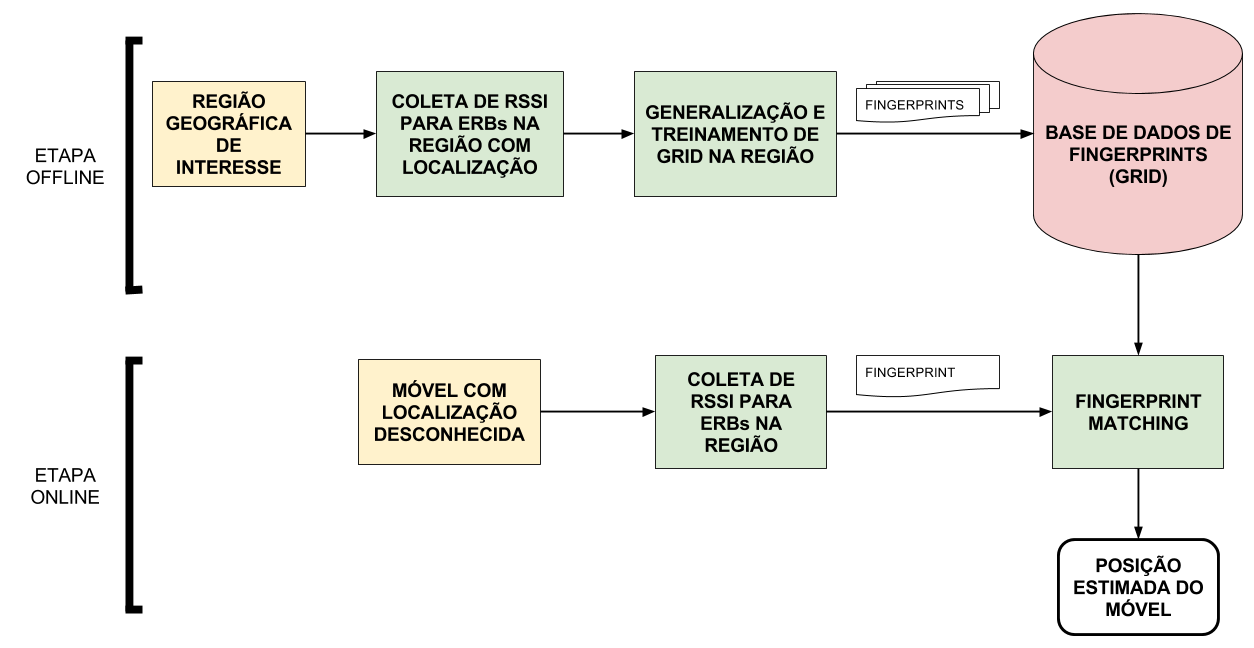
\includegraphics[width=16cm]{images/arquiteturaFpRSSI.png}\par
                \caption{Modelo de arquitetura de \textit{fingerprinting} com RSSI utilizando GRIDs.}
                \label{fig:arquiteturaFingerprintingRSSI}
            \end{figure}

                %------------------------------------
                % ETAPA - COLETA DE AMOSTRAS
                \subsubsubsection{Coleta de Amostras de RSSI}
                \label{sec:coletaAmostras}

				A criação da base de dados de \textit{fingerprints} necessita de informações de RSSI para as ERBs da região de interesse. Uma das desvantagens da técnica de \textit{fingerprinting} utilizando RSSI é que os níveis de sinal no ambiente urbano variam com o passar do tempo por diversos fatores como por exemplo alterações na antenas da rede celular e o efeito multipath, isso implica que as medições devem ser refeitas após um período de tempo ou do contrário o sistema de localização irá perder precisão.
				
				Um dos métodos mais conhecidos para coletar esta informação é o \textit{Wardriving}, que consiste em deslocar-se pela região de interesse (em geral utilizando um automóvel) com um dispositivo provido de GPS e uma interface de rádio capaz de sentir o nível de sinal para cada ERB. Esta prática pode demandar grande esforço especialmente se a região de interesse possuir uma área muito extensa, além de gerar medições apenas em ruas dependendo do meio de transporte utilizado (um estudo interessante sobre a acurácia dessa técnica pode ser encontrado em \cite{wardriving2010}). 
				
				É possível utilizar modelos matemáticos para prever os níveis de sinal como mostrado em \cite{teseRobson2014}. A vantagem dessa abordagem é que não necessita esforço de coleta porém, em geral, as medições empíricas geram modelos mais precisos por utilizarem valores reais, além disso, alguns modelos podem demandar um grande esforço computacional para gerar boas simulações.

                %------------------------------------
                % ETAPA - TREINAMENTO DO GRID
                \subsubsubsection{Formação do GRID de \textit{Fingerprints}}
                \label{sec:treinamentoGRIDs}

				A maneira com que são armazenados os \textit{fingerprints} da base de dados é subdividindo a região de interesse em um GRID de células menores em que cada \textit{fingerprint} possui a localização do centro de sua célula. Esses GRIDs podem ser regulares ou irregulares.
				
				GRIDs Regulares, como o mostrado na Figura \ref{fig:gridRegular}, são caracterizados por possuirem formato retangular e espaçamentos regulares entre as suas células. O número de células necessárias para cobrir uma região depende da aŕea da região e da resolução utilizada. Quanto maior a resolução, maior a precisão para os móveis que se encontram na área porém exige um custo computacional maior devido ao grande número de células geradas (um estudo sobre isso pode ser encontrado em \cite{gridResolutionImpact2011}). 
				
				GRIDs Irregulares (como o mostrado em \cite{unevenGridFingerprinting2015}) por outro lado, podem assumir formas variadas e são geralmente mantidos como uma lista de pontos que representam os centros de suas células.
				
				\begin{figure}[H]
                \centering
                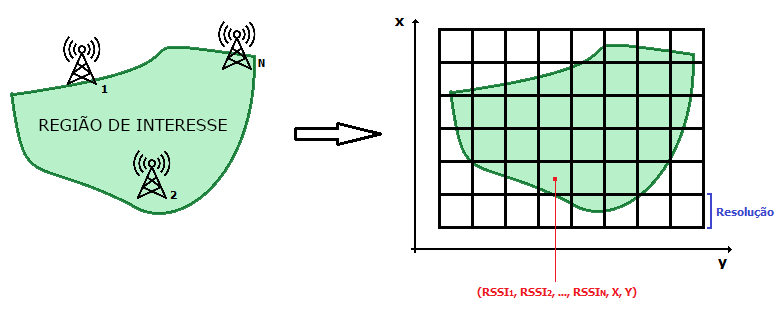
\includegraphics[width=14cm]{images/gridRegular.png}\par
                \caption{Mapeamento de região utilizando um GRID regular.}
                \label{fig:gridRegular}
                \end{figure}
				
				As medições de RSSI coletadas podem ser utilizadas diretamente para se montar um GRID, seja regular ou irregular, porém, obter informações suficientes para cobrir toda a área de interesse em geral necessitaria de muitas amostras e um extenso trabalho de coleta. Uma solução para isso é utilizar as medições feitas apenas como base para a construção do GRID, prevendo os níveis de sinal em cada célula com uma abordagem de regressão por técnicas aprendizado de máquina supervisionadas (ver Seção \ref{sec:aprendizadoDeMaquina} para mais detalhes sobre regressão).
				
				\begin{figure}[H]
                \centering
                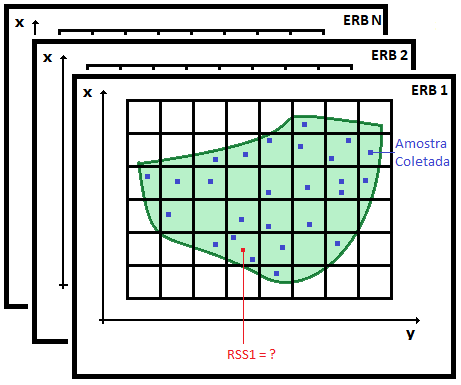
\includegraphics[width=14cm]{images/regressaoFingerprinting.png}\par
                \caption{Regressão de maneira a descobrir os níveis de sinal no centro de cada célula do GRID a partir das amostras coletadas.}
                \label{fig:regressaoFingerprinting}
                \end{figure}
				
				A Figura \ref{fig:regressaoFingerprinting} ilustra o processo de treinamento. O processo completo que será utilizado para este trabalho está descrito no algoritmo 1. Para cada padrão de treinamento, as coordenadas geográficas são utilizadas como atributos de entrada e a saída é dada pelo nível de sinal detectado para a ERB em questão, assim, é gerado um modelo do comportamento cada ERB na região de interesse a partir da base de dados de medições e com esses modelos é possível prever o nível de sinal nos centros de cada célula.
                        
                        %ALGORITMO - Treinamento de GRIDs
                        \vspace*{5mm}
                        \begin{algorithm}[H]
                            \label{alg:treinamentoGrid}
                            \caption{\textsc{Treinamento de GRID}.}
                            \SetAlgoLined
                            
                            \Entrada{
                                Conjunto S de modelos de aprendizado de cada ERB da região,
                                Conjunto T de amostras de treinamento disponíveis,
                                Conjunto C de células do GRID.
                            } 
                            
                            \Saida{GRID de células C com estimativas de RSSI para cada ERB }
                            \vspace*{3mm}
                            //Treinamento dos modelos de aprendizado\\
                            Para cada ERB $e$ da região:\\
                            \Inicio{
                                Treina o modelo da ERB com T de maneira que para cada amostra t de T:\\
                                $X_t = [latitude_t, longitude_t]$ \\
                                $Y_t = RSSI_{t,e}$ \\
                            }
                            \vspace*{3mm}
                            //Treinamento do GRID de células\\
                            Para cada célula $c$ de C:\\
                            \Inicio{
                                Para cada ERB $e$ da região:\\
                                $RSSI_{c,e} = S_e(latitude_c, longitude_c)$\\
                            }
                        \end{algorithm}
                        \vspace*{5mm}
				
				O foco deste trabalho nos próximos Capítulos será verificar a diferença de desempenho do sistema de localização utilizando algoritmos diferentes para executar a regressão no treinamento de um GRID de células regular.
				
                %------------------------------------
                % ETAPA - ESTIMAR POSIÇÃO FAZENDO MATCHING
                \subsubsubsection{Algoritmo de \textit{Matching} para Estimar a posição do móvel}
                \label{sec:algoritmoMatching}

                A etapa de \textit{matching} do \textit{fingerprinting} consiste em encontrar a célula cujo identificador mais se assemelha com o identificador gerado para o dispositivo móvel em sua localização atual.
                
                Existem diversos algoritmos para fazer \textit{matching} baseado em similaridade, \cite{handbookPositionLocation2012} mostra uma abordagem utilizando uma Rede Neural Artificial que tem como entrada os níveis de sinal detectados no móvel e saída a célula mais compatível do GRID.
                
                Uma abordagem simples porém eficaz e que será utilizada nos próximos Capítulos é atribuir uma função de similaridade que possua como entrada 2 \textit{fingerprints} e como saída um valor representando a compatibilidade entre eles. Pode-se definir então a similaridade geral entre 2 \textit{fingerprints} $a$ e $b$ através da seguinte equação:
                
                \begin{equation} 
                \label{eq:similaridadeGeral}
                S(a,b) = \sum_{i=1}^{n} s(a_{i}, b_{i})~,
                \end{equation}
                
                \noindent em que a similaridade total $S(a, b)$ é dada pela soma das similaridades parciais $s(a_{i}, b_{i})$ para cada uma das $n$ ERBs do sistema. Essa função $s$ varia de acordo com o algoritmo de distância escolhido. Utilizando a tradicional Distância Euclidiana, a similaridade entre dois \textit{fingerprints} com relação a apenas uma ERB seria: 
                
                \begin{equation}
                \label{eq:similaridadeEuclidianaParcial}
                s(a_{i}, b_{i}) = \sqrt{(RSSI_{a,i} - RSSI_{b,i})^2}~,
                \end{equation}
                
                \noindent em que $RSSI_{a,i}$ e $RSSI_{b,i}$ representam os níveis de sinal em relação a ERB $i$ sentidos pelos \textit{fingerprints} $a$ e $b$ respectivamente. Essa distância poderia ser substituída por outras métricas presentes na literatura como por exemplo a Distância Manhattan ($s(a_{i}, b_{i}) = |RSSI_{a,i} - RSSI_{b,i}|$). Diferentes distâncias podem mudar completamente o resultado do algoritmo de \textit{matching}. 
                
                O valor da similaridade $S$ total entre dois \textit{fingerprints} será menor quanto mais compatíveis são os \textit{fingerprints} em questão. Utilizando distância euclidiana, $S$ seria então representada pela equação abaixo:
                
                \begin{equation} 
                \label{eq:similaridadeEuclidiana}
                S(a,b) = \sum_{i=1}^{n} \sqrt{(RSSI_{a,i} - RSSI_{b,i})^2} 
                \end{equation}
                
                O algoritmo de \textit{matching} portanto precisa calcular a similaridade entre o \textit{fingerprint} do móvel e cada \textit{fingerprint} da base de dados e selecionar a célula com menor valor de $S$ como a célula mais compatível e portanto mais provável de representar a localização do móvel.
                
                Vale notar que, como mencionado anteriomente, o aumento da resolução do GRID acarreta em um maior número de células para se calcular e comparar a similaridade e portanto um maior custo computacional. Nessa abordagem, dependendo do tamanho da região, é recomendável executar algum tipo de filtro de células antes de executar o algoritmo de \textit{matching} para melhorar o desempenho do algoritmo. Como por exemplo utilizar apenas células próximas à ERB fornecedora atual de serviço para o móvel.  

        %------------------------------------
        % ALGORITMOS DE APRENDIZADO DE MÁQUINA UTILIZADOS
        \subsection{Algoritmos de Aprendizado de Máquina Supervisionados para Regressão}
        \label{sec:aprendizadoDeMaquina}
        
        Para executar a tarefa de treinamento dos GRIDs regulares de maneira supervisionada (com conhecimento prévio da resposta desejada nos exemplos de treino) mostrada na Seção \ref{sec:treinamentoGRIDs}, são utilizados algoritmos de aprendizado de máquina supervisionados para realizar o processo conhecido como regressão, que consiste de a partir de um conjunto de atributos $X = [x_1, x_2, ..., x_n]$ estimar a resposta $Y$ do sistema. A diferença entre regressão e o problema de classificação é que enquanto o segundo obtém como resposta uma classe entre um conjunto discreto de classes definidas a regressão obtém um valor de saída representado por um número real. 
        
        As Seções a seguir irão abordar alguns algoritmos mais conhecidos de aprendizado de máquina capazes de executar a tarefa de regressão mencionada e que serão utilizadas no Capítulo \ref{sec:metodologia}. Esses algoritmos representam diferentes classes de regressores e seus desempenhos dentro do cenário de localizaçãoa serão avaliados nos próximos capítulos. 
        
            %------------------------------------
            % KNN
            \subsubsection{K Vizinhos Mais Próximos (KNN)}
            \label{sec:KNN}

            O algoritmo K vizinhos Mais Próximos é um dos algoritmos mais simples em termos de implementação porém pode obter bons resultados em diversas aplicações.
            
            Essa é uma técnica baseada em instâncias (ver \cite{instanceBasedLearning1991}), isto é, não necessita de treinamento prévio. Durante a execução do algoritmo, são selecionadas as $K$ amostras da base de dados que possuam o conjunto de atributos mais similar ao da nova amostra que se quer determinar a saída. Baseado nos valores de saída $Y$ das $K$ amostras, é estimado o valor de saída $Y$ da nova amostra.
            O algorítmo KNN possui muitas variações diferentes porém a sua forma mais geral utiliza distância euclidiana como medida de similaridade entre amostras e média aritmética das saídas das $K$ amostras como a saída para a nova amostra.
            
            \begin{figure}[H]
            \centering
            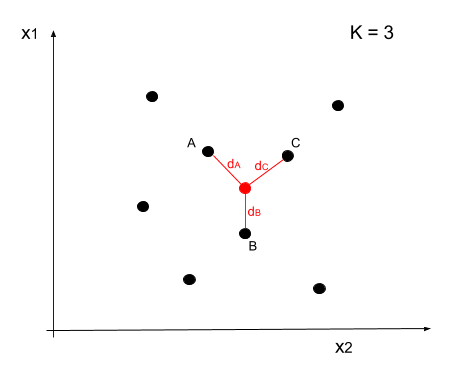
\includegraphics[width=10cm]{images/KNN.png}\par
            \caption{Exemplo de KNN com apenas 2 atributos e $K$ = 3.}
            \label{fig:exemploKNN}
            \end{figure}
            
            Uma modificação bastante interessante de ser feita no algoritmo básico é utilizar uma média aritmética ponderada pela distância entre amostras no lugar da média aritmética simples para estimar o valor de saída (\cite{wknn2004}). Isso permite que amostras que estejam mais próximas da nova amostra possuam maior importância que as amostras mais distantes na decisão do valor de saída. A nova fórmula da saída $Y$ considerando cada atributo $x_i$ do vetor de atributos $X$ da amostra e sua respectiva distância $d_i$ em relação ao mesmo atributo da nova amostra seria:
            
            \begin{equation} 
            \label{eq:mediaPonderada}
            Y = \frac{\sum_{i=1}^{n} x_i (\frac{1}{d_i})^W}
                {\sum_{i=1}^{n} (\frac{1}{d_i})^W}
            \end{equation}
            
            \noindent Nessa equação foi adicionado também um novo parâmetro $W$ que define o grau de importância da distância $d_i$ no valor da média. Quanto maior o valor de $W$ maior é a importância da distância de cada vizinho no valor de saída. Vale notar que se $W = 0$ então a fórmula se torna uma média aritmética simples.
            
            Embora simples de implementar, este algoritmo possui uma  desvantagem principal. Para descobrir quem são os $K$ vizinhos mais próximos da amostra com saída desconhecida, é necessário calcular e comparar a distância até cada amostra presente na base de dados, o que significa um custo $O(N)$ para o número $N$ de amostras da base de dados. Dependendo da aplicação, essa pode ser uma desvantagem crucial em relação a outros algoritmos que embora possuam um tempo de treinamento \textit{offline} elevado podem executar a regressão \textit{online} em muito menos tempo.  
            
            %------------------------------------
            % MLP
            \subsubsection{\textit{Perceptron Multicamadas (MLP)}}
            \label{sec:MLP}

            O \textit{Perceptron} Multicamadas trata-se de um modelo de Rede Neural Artificial (\textit{Artificial Neural Network}, ANN) capaz de extrair informações de amostras de treinamento e armazenar nos pesos de um conjunto de unidades ou neurônios que formam a rede neural. Esta abordagem possui inspiração biológica e é utilizada em diversas aplicações.
            
            As unidades do MLP são os neurônios conhecidos como \textit{Perceptrons}. Cada \textit{Perceptron} por sí só pode atuar como uma máquina de aprendizado muito simples, capaz apenas de executar regressões lineares e resolver problemas de classificação linearmente separáveis. A Figura \ref{fig:perceptron} mostra o modelo de funcionamento de um \textit{Perceptron}:
            
            \begin{figure}[H]
            \centering
            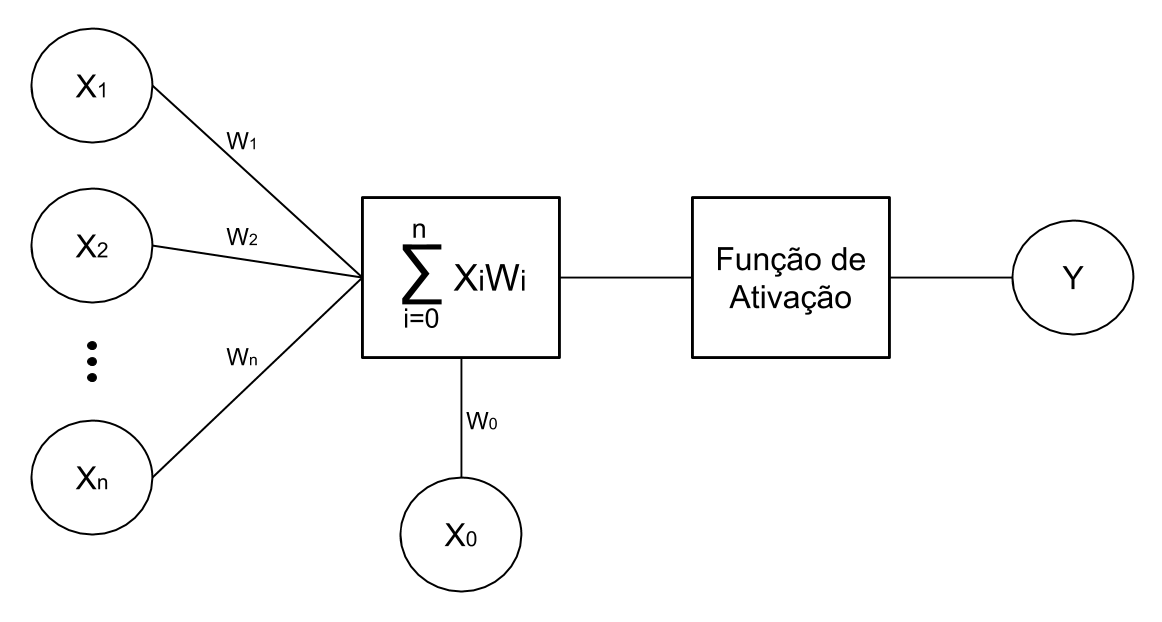
\includegraphics[width=14cm]{images/perceptron.png}\par
            \caption{Modelo de neurônio \textit{Perceptron}.}
            \label{fig:perceptron}
            \end{figure}
            
            Esta célula possui um vetor de entrada $X = [x_1, x_2, ..., x_n]$ e este vetor é combinado linearmente a um vetor de pesos $W = [w_1, w_2, ..., w_n]$ e somados à uma entrada constante ou \textit{bias} (modelado muitas vezes como a constante $\theta$ ou uma entrada constante $x_0$ associada a um peso $w_0$) para gerar uma resposta para o sistema. Esta combinação passa por uma função de ativação que possui importante papel em problemas de classificação mas pode ser substituída pela função identidade para problemas de regressão, e gerar o resultado $Y$ da regressão. 
            
            O vetor de pesos $W$ do \textit{Perceptron} em geral é inicializado de maneira aleatória e o objetivo do treinamento do modelo com a base de dados de amostras é determinar o valor de cada peso de entrada e o peso do \textit{bias} que obtenham os valores desejados de $Y$.
            
            A rede MLP surge como uma solução para superar as limitações do \textit{Perceptron}. A Figura \ref{fig:MLP} mostra o esquemático de arquitetura geral de uma rede MLP. Trata-se de uma rede do tipo \textit{Feedfoward} totalmente conectada, isto é, o grafo de conexões não forma um ciclo e cada neurônio de uma camada é conectado a todos os neurônios da camada seguinte. 
            
            \begin{figure}[H]
            \centering
            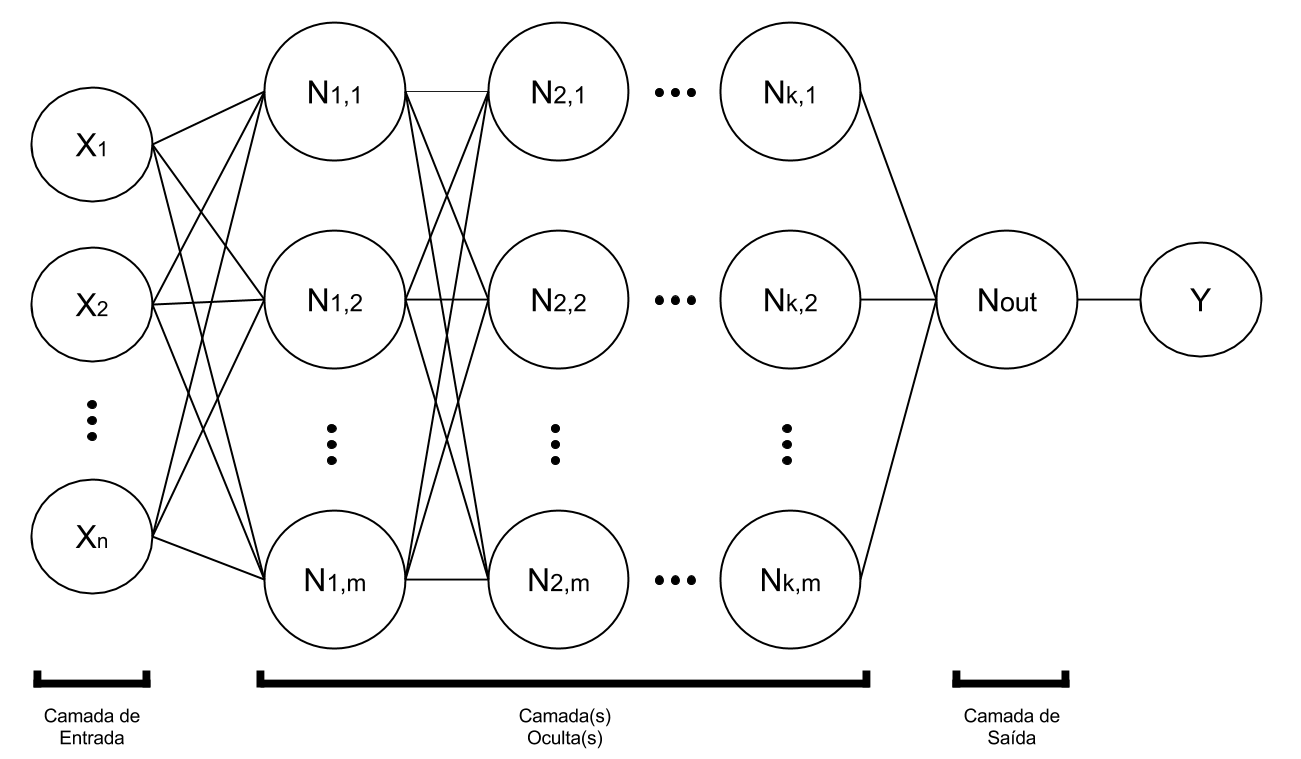
\includegraphics[width=16cm]{images/MLP.png}\par
            \caption{Modelo genérico de rede neural MLP.}
            \label{fig:MLP}
            \end{figure}
            
            As 3 camadas que constituem a rede são a camada de entrada, a camada (ou camadas) oculta e a camada de saída. A camada de entrada consiste simplesmente do vetor de entrada $X$. A camada de saída é um \textit{Perceptron} utilizando em geral a função identidade para regressão. As camadas ocultas não possuem contato com a saída final $Y$ e formam a parte interna da rede, sendo constituídas de \textit{Perceptrons} utilizando alguma função não-linear como função de ativação (tipicamente a função sigmoid $ f(x) = \frac{L}{1+e^{-k()x-x_0}} $) para que a rede tenha a capacidade de representar até mesmo funções altamente não-lineares.
            
            O algoritmo clássico para treinar uma rede neural MLP é o \textit{Backpropagation}. O treinamento ocorre iterativamente por todas as amostras de treino em que cada vez que a rede erra o resultado de uma amostra (no caso de uma regressão, quando o valor obtido é diferente do valor desejado acima de um certo limiar) é aplicado o \textit{Backpropagation}. O treinamento encerra quando a rede obtém um desempenho aceitável ou supera um determinado número máximo de iterações. 
            
            Também é utilizado um parâmetro conhecido como taxa de aprendizado (ou \textit{Learning Rate}), que regula o tamanho do ajuste nos pesos a cada vez que a rede erra o resultado para uma amostra. Essa taxa pode ser um valor constante, pode ser um valor dinâmico que diminui com o passar do tempo para obter maior precisão, etc.
            
            O algoritmo \textit{Backpropagation} em si tenta minimizar o erro quadrático entre a saída obtida e a saída desejada através de Gradiente Descendente. Uma derivação completa do algoritmo pode ser encontrada em \cite{machineLearning1997}.
            
            %------------------------------------
            % SVM
            \subsubsection{Máquina de Vetores de Suporte (SVM)}
            \label{sec:SVM}

            O algoritmo de Máquina de Vetores de Suporte foi desenvolvido a mais de cinquenta anos atrás porém só recentemente ganhou popularidade em várias aplicações, como classificação de imagens e detecção de caracteres (\cite{applicationsSVM} contém uma lista com essas e muitas outras aplicações bastante interessantes desse algoritmo). Originalmente as SVMs só eram capazes de solucionar problemas linearmente separáveis porem \cite{svm1992} de 1992, mostrou a capacidade das SMVs de resolver problemas mais complexos utilizando Kernels não lineares.
            
            Seja o problema bidimensional exemplo da Figura \ref{fig:SVM} linearmente separável, existe pelo menos um hiperplano do tipo $Y(X) = W.X + b = 0$ capaz de separar completamente as duas classes. O que a SVM faz é tentar encontrar o melhor hiperplano, isto é, aquele que deixa a maior margem até a primeira amostra de cada classe (conhecidos como os vetores de suporte).
            
            De posse desse hiperplano é possível fazer a classificação de um novo padrão de maneira muito simples e extremamente eficiente em termos de processamento apenas utilizando o vetor de atributos $X$ do novo padrão e tendo como resultado a primeira classe se $Y(X) > 0$ e a segunda classe se $Y(X) < 0$ (o caso em que $Y(X) = 0$ é considerado o limiar de decisão e pode ser decidido arbitrariamente). Dessa forma o treinamento desta máquina de aprendizado consiste em descobrir o valor dos parâmetros vetor e \textit{bias} $W$ e $b$ da equação.
            
            \begin{figure}[H]
            \centering
            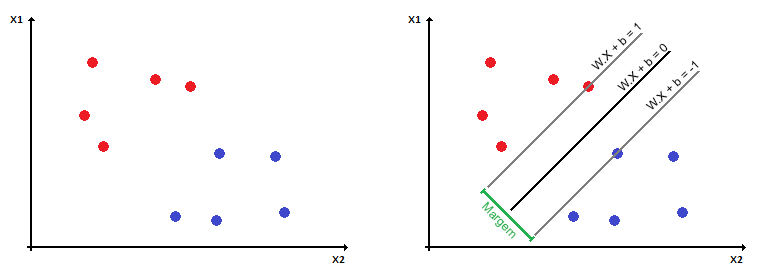
\includegraphics[width=16cm]{images/SVM.png}\par
            \caption{Exemplo de divisão por hiperplano de uma SVM.}
            \label{fig:SVM}
            \end{figure}
            
            Considerando que a classe positiva para qualquer amostra $n$ terá $W.X_n + b >= 1$ e definindo sua classificação esperada como $Y_n = +1$. A classe negativa por sua vez terá classificação $Y_n = -1$ e obedecerá $W.X_n + b <= -1$. Portanto, qualquer amostra de qualquer classe seguirá a restrição: 
            
            \begin{equation} 
            \label{eq:svmRestricao}
            Y_n(W.X_n + b) >= 1
            \end{equation}
            
            Já a margem entre o hiperplano de decisão e as amostras mais próximas de cada classe é dada por:
            
            \begin{equation} 
            \label{eq:svmMargem}
            margem = \frac{2}{||W||}
            \end{equation}
            
            Dessa forma, para encontrar $W$ e $b$ que maximizem a margem é preciso minimizar $||W||$ seguindo a restrição de classificação imposta pela Inequação \ref{eq:svmRestricao}. Como a Equação \ref{eq:svmMargem} pode ser reescrita por $\frac{1}{2}||W||^2$ então, este trata-se de um problema de otimização convexo para minimizar uma função quadrática com uma restrição linear. Sendo convexo, o problema possui apenas um ponto de mínimo que é o mínimo global. Uma análise mais aprofundada do problema de otimização das SVMs e soluções existentes pode ser encontrada em \cite{svmSolvers2007}.
            
            Para impedir o \textit{overfitting} e permitir uma melhor generalização do modelo, a restrição \ref{eq:svmRestricao} pode ser relaxada introduzindo-se um parâmetro de tolerância $\epsilon$. Este parâmetro é conhecido como \textit{slack} e possui valor $0 <= \epsilon <= 1$. Quanto maior o seu valor, mais permissivo é o modelo. A nova restrição se torna então:
            
            \begin{equation} 
            \label{eq:svmRestricaoSlack}
            Y_n(W.X_n + b) >= 1 - \epsilon
            \end{equation}
            
            A introdução de $\epsilon$ implica na alteração da equação que se deseja minimizar pois agora também será necessário minimizar a soma dos valores de erro de cada amostra devido ao \textit{slack}. A nova equação a ser minimizada será:
            
            \begin{equation} 
            \label{eq:svmSlack}
            \frac{1}{2}||W||^2 + C\sum_n{\epsilon_{n}}~,
            \end{equation}
            
            \noindent essa equação também introduz um coeficiente $C$ que denota a importância da punição por violações da margem pelas amostras para a otimização. Quanto maior o valor de C, mais rígida se torna a margem.
            
            Para permitir a solução de problemas não linearmente separáveis \cite{svm1992} utiliza Kernels não lineares para levar o conjunto de dados para um espaço vetorial com mais dimensões em que este conjunto seja linearmente separável. A equação do hiperplano portanto é alterada de maneira que se adicione uma transformação $\phi$ no vetor de atributos $X$:
            
            \begin{equation} 
            \label{eq:svmTransformation}
            Y(X) = W.\phi(X) + b = 0~,
            \end{equation}
            
            \noindent em que é possível aplicar o \textit{Kernel Trick} da seguinte equação para aplicar a transformação $\phi(X)$ sem conhecê-la utilizando um Kernel $K(X_i, X)$: 
            
            \begin{equation} 
            \label{eq:svmKernelTrick}
            W.\phi(X) = \sum_{i}{\alpha_{i}Y_{i}K(X_i, X) }
            \end{equation}
            
            Existem diversos Kernels porém alguns dos mais populares são o Polinomial, o Sigmoid e RBF (\textit{Radial Basis Function}). Uma explicação detalhada pode ser encontrada em \cite{patternRecognition1997}.
            
            Até agora foi mostrado o funcionamento de SVMs para o problema de classificação para um melhor entendimento, porém, SVMs também são capazes de executar regressão. A variação do algoritmo que para isso será utilizada ao longo deste trabalho é a \textit{Support Vector Regression} ou SVR, introduzida por \cite{svr1997}. Neste modelo as restrições utilizadas para cada amostra são:
            
            \begin{equation} 
            \label{eq:svrRestriction1}
            Y_n - W \times X_n - b <= \epsilon ~,
            \end{equation}
            
            \begin{equation} 
            \label{eq:svrRestriction2}
            W \times X_n + b - Y_n <= \epsilon ~,
            \end{equation}
            
            \noindent em que $\epsilon$ é um limiar estabelecido e a predição de valor $Y(X)$ pode ser feita através de $W \times X_n + b$.
            
            %------------------------------------
            % RANDOM FOREST
            \subsubsection{\textit{Random Forest}}
            \label{sec:randomForest}

            A última técnica que será utilizada neste trabalho se chama \textit{Random Forest} (Floresta Aleatória). Assim como o \textit{Perceptron} Multicamadas, \textit{Random Forests} são compostas por outras estruturas menores que por si só são também máquinas de aprendizado. Essas estruturas são conhecidas com Árvores de Decisão (\textit{Decision Trees}) e podem ser utilizadas tanto para classificação quanto regressão.
            
            Uma Árvore de Decisão trata-se de um grafo acíclico em formato de árvore invertida em que, iniciado por um nó raiz, cada nó seleciona um atributo $X_i$ do vetor de entrada $X$ e gera nós filhos separando o conjunto de amostras de treinamento do nó pai em subconjuntos de acordo com o valor $X_i$ de cada amostra. Os nós mais profundos são conhecidos como folhas e contém a classe ou valor final (no caso de regressão) ao seguir um determinado caminho na árvore e não há mais atributos para selecionar.
            
            \begin{figure}[H]
            \centering
            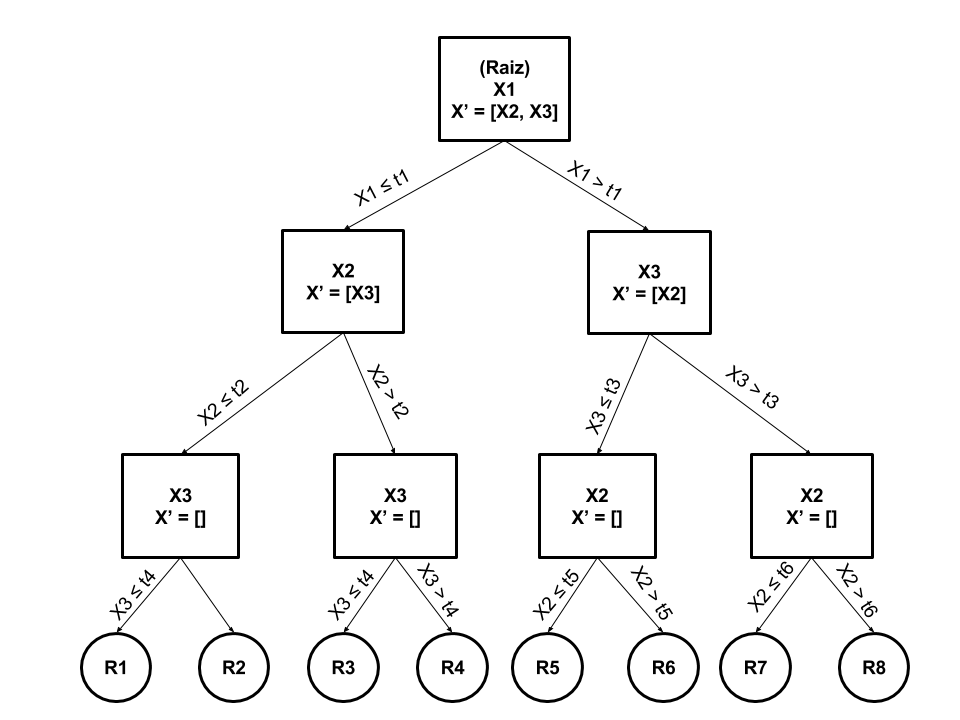
\includegraphics[width=16cm]{images/arvoreDecisao.png}\par
            \caption{Exemplo de uma Árvore de Decisão em um problema com 3 atributos.}
            \label{fig:decisionTree}
            \end{figure}
            
            As Árvores de Decisão utilizadas para regressão como a da Figura \ref{fig:decisionTree} são binárias por selecionar valores maiores e menores do que um limiar e selecionam o atributo para particionar de maneira a minimizar o erro médio quadrático entre os valores de saída desejada Y de cada amostra dos subconjuntos resultantes de amostras $R_1 e R_2$ e a média das saídas desejadas para cada subconjunto. Esse erro é dado pela seguinte equação:
            
            \begin{equation} 
            \label{eq:decisionTreeMinimize}
            \sum_{p \in R_1}{(Y_p - Mean(Y_{R_1}))^2} +
            \sum_{p \in R_2}{(Y_p - Mean(Y_{R_2}))^2}~,
            \end{equation}
            
            \noindent em que $Mean$ representa a função média aritmética e $Y_{R_1}$ e $Y_{R_2}$ representam os conjuntos de valores $Y$ para a região 1 e região 2 respectivamente. 
            
            Um dos problemas com Árvores de Decisão é que sua construção por completo tende a causar o \textit{overfitting} do modelo, isto é, a máquina decora os padrões de treinamento. Uma das soluções para resolver esse problema é fazer a poda ou \textit{prunning} da árvore para impedir que se expanda por completo e permita maior generalização do problema. 
            
            O algoritmo de \textit{Random Forest} tenta reduzir o problema de \textit{overfitting} além de gerar melhores predições através do uso de várias Árvores de Decisão criadas utilizando a mesma base de dados.
            
            No treinamento de uma \textit{Random Forest} um número $M$ de árvores é gerado com a base de dados de amostras porém a ordem de particionamento nos nós é aleatória em cada árvore ao invés de minimizar o erro quadrático (daí o nome da técnica). Isso reduz a correlação entre as árvores e as torna mais resistentes a ruídos na base de dados. A regressão então, é executada de maneira muito simples (como ilustrado pela Figura \ref{fig:randomForest}) apenas verificando o valor resultante de cada árvore e fazendo uma média aritmética destes resultados.

            \begin{figure}[H]
            \centering
            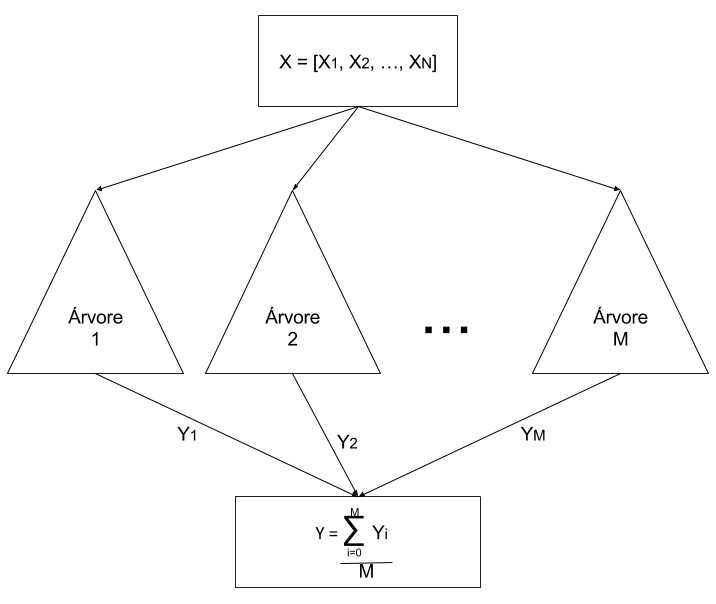
\includegraphics[width=16cm]{images/randomForest.png}\par
            \caption{Regressão utilizando \textit{Random Forest}.}
            \label{fig:randomForest}
            \end{figure}

    %------------------------------------
    % METODOLOGIA E RESULTADOS
    \newpage
    \section{Metodologia e Resultados}
    \label{sec:metodologia}
    
    Este Capítulo detalha o experimento que foi executado. Ele consiste de maneira geral em construir GRIDs regulares de diferentes resoluções a partir de uma base de amostras de RSSI e treinar cada GRID utilizando os algoritmos apresentados na Seção \ref{sec:aprendizadoDeMaquina}, tendo seus parâmetros de aprendizado variados. A implementação foi feita utilizando linguagem de programação \textit{Python} e a biblioteca de aprendizado de máquina \textit{Scikit Learn} 0.18 (\cite{scikitLearn}). Serão apresentadas métricas de desempenho e por fim será feita uma análise comparativa dos resultados obtidos.

        %------------------------------------
        % BASE DE DADOS
        \subsection{Base de Amostras Utilizada}
        \label{sec:experimentoBaseDeDados}

        Para os experimentos a seguir foi utilizada uma base de dados com 2956 medições de RSSI em $DB_m$ para 6 ERBs em uma área urbana de aproximadamente 5 $km^2$ na cidade do Recife em Pernambuco - Brasil. 
        
        Essa mesma base de dados foi utilizada em \cite{teseRobson2014} e suas medições foram coletadas por \textit{wardriving} utilizando o receptor modular de escaneamento digital de intensidade de sinais de radiofrequência NEMO FS R1.
        
        Uma visualização das amostras contidas na base de dados encontra-se na Figura \ref{fig:visualizacaoAmostras} na qual é possível verificar a posição de uma das ERBs (indicada pelo triângulo preto) e níveis de sinal até ela variando de tons verdes (mais fracos) até tons vermelhos (mais fortes).
        
        \begin{figure}[H]
        \centering
        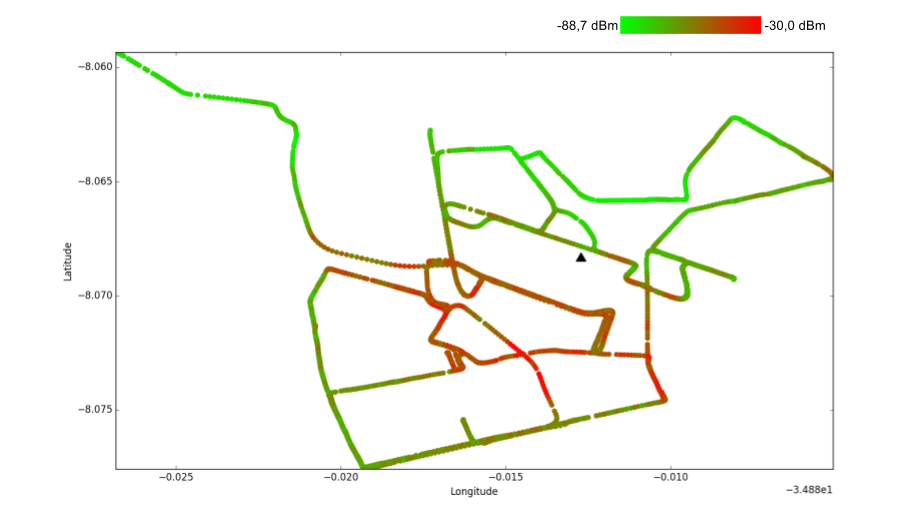
\includegraphics[width=16cm]{images/visualizacaoAmostras.png}\par
        \caption{Visualização de amostras da base e seus níveis de sinal para a ERB 1.}
        \label{fig:visualizacaoAmostras}
        \end{figure}
    
        %------------------------------------
        % CONSTRUÇÃO DO GRID REGULAR
        \subsection{Construção do GRID Regular}
        \label{sec:experimentoGrid}
        
        A construção do GRID regular a partir da base de amostras teve duas etapas. Na primeira foram escolhidas as coordenadas dos centros de cada célula do GRID de maneira a cobrir toda a área em que as amostras estavam contidas e espaçando as células de acordo com a resolução escolhida. Para o experimento foram gerados GRIDs com 3 resoluções diferentes: 10, 20 e 30 metros.
        
        Na segunda etapa, os GRIDs foram treinados para se obter a estimativa de RSSI para cada ERB em cada célula a partir do processo descrito pelo Algoritmo \ref{alg:treinamentoGrid} na Seção \ref{sec:treinamentoGRIDs}.
        
        Os GRIDs resultantes estão em formato como o da Figura \ref{fig:visualizacaoGrid}. Nela pode-se ver a tentativa de generalização de uma máquina de aprendizado obtendo um mapeamento completo dos níveis de sinal da região mesmo em pontos sem amostras coletadas por perto.
        
        \begin{figure}[H]
        \centering
        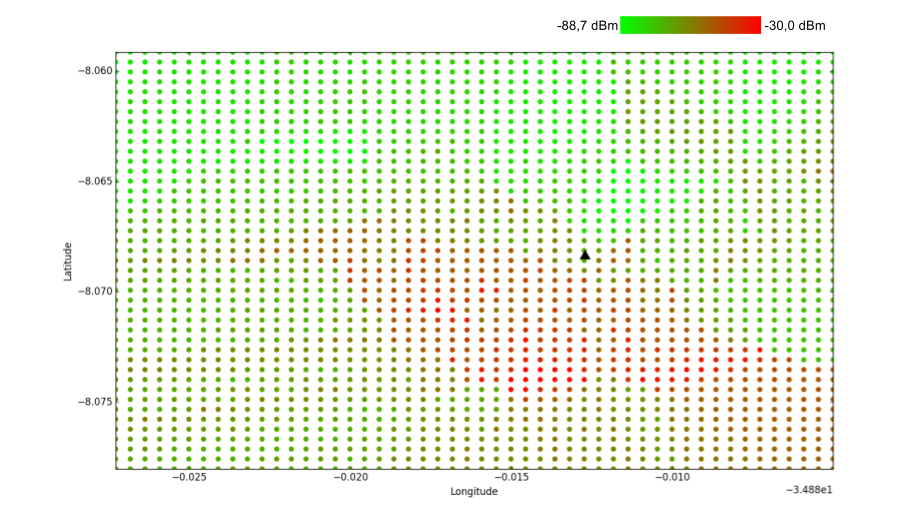
\includegraphics[width=16cm]{images/visualizacaoGrid.png}\par
        \caption{Visualização de GRID com resolução de 50m treinado em relação à ERB 1 com KNN($K=4$, $W=1$).}
        \label{fig:visualizacaoGrid}
        \end{figure}
        
        Um ponto importante a se notar é o crescimento exponencial do número de células necessárias para se cobrir a região ao modificar a resolução. Um GRID com 30m de resolução resultou em 5740 células enquanto que 20m resultou em 12688 células e um GRID de 10m de resolução resultou em 49610 células. 
        
        %------------------------------------
        % ALGORITMOS DE REGRESSÃO
        \subsection{Algoritmos de Regressão}
        \label{sec:experimentoParametros}
        
        Os algoritmos apresentados na Seção \ref{sec:aprendizadoDeMaquina} foram utilizados como modelos para estimar valores de RSSI. Cada algoritmo possui parâmetros específicos que podem ser variados para melhorar o desempenho dos modelos. A seguir serão listados os parâmetros de cada algoritmo e faixa de valores utilizados para estes parâmetros. 
        
        A variação do algoritmo KNN utilizada possui 2 parâmetros: o número $K$ de vizinhos mais próximos selecionados e o valor $W$ que define a importância da distância de cada vizinho até a nova amostra na média ponderada.
        
        %TABELA KNN
        \begin{table}[htb]
        \centering
        \caption{Parâmetros Utilizados - KNN.}
        \label{table:parametersKNN}
        \begin{tabular}{ | l | p{5cm} |}
        \hline
        \textbf{Parâmetro} & \textbf{Valores} \\ \hline
        $K$ & 0; 1; 2; 3; 4; 5 \\ \hline
        $W$ & 0; 1; 2; 3 \\ \hline
        \end{tabular}
        \end{table}
        
        Para o MLP foram utilizados os seguintes parâmetros: função de ativação das camadas ocultas (na tabela relu e tanh significam função linear unitária retificada e tangente hiperbólica respectivamente); o número de unidades na camada oculta; o tipo da taxa de aprendizado, que pode ser constante, reduzir com o tempo (\textit{invscaling}) ou adaptativo de acordo com o treinamento. A taxa de aprendizado inicial utilizada foi 0,001.
        
        %TABELA MLP
        \begin{table}[htb]
        \centering
        \caption{Parâmetros Utilizados - MLP}
        \label{table:parametersMLP}
        \begin{tabular}{ | l | p{7cm} |} \hline
        \textbf{Parâmetro} & \textbf{Valores} \\ \hline
        Função de Ativação (Act) & identidade; logistica; tanh; relu \\ \hline
        Taxa de Aprendizado (LR) & constante; invscaling; adaptativo \\ \hline
        Tamanho da Camada Oculta (HLS) & 50; 100; 200; 500 \\ \hline
        \end{tabular}
        \end{table}
        
        Os parâmetros utilizados para as SVMs foram o tipo de Kernel utilizado, o parâmetro \textit{slack} $\epsilon$ e o parâmetro de penalização $C$. 
        
        %TABELA SVM
        \begin{table}[htb]
        \centering
        \caption{Parâmetros Utilizados - SVM.}
        \label{table:parametersSVM}
        \begin{tabular}{ | l | p{7cm} |} \hline
        \textbf{Parâmetro} & \textbf{Valores} \\ \hline
        Kernel & polinomial; rbf; linear; sigmoid \\ \hline
        C & 0,5; 1; 2; 5 \\ \hline
        $\epsilon$ & 0,05; 0,1; 0,2; 0,5 \\ \hline
        \end{tabular}
        \end{table}
        
        Para o \textit{Random Forest} o único parâmetro utilizado é o número $M$ de árvores de decisão da floresta.
        
        %TABELA RANDOM FOREST
        \begin{table}[!ht]
        \centering
        \caption{Parâmetros Utilizados - \textit{Random Forest}.}
        \label{table:parametersRF}
        \begin{tabular}{ | l | l | } \hline
        \textbf{Parâmetro} & \textbf{Valores} \\ \hline
        $M$ & 10; 20; 50; 75; 100 \\ \hline
        \end{tabular}
        \end{table}
            
        %------------------------------------
        % MÉTRICAS DE DESEMPENHO
        \subsection{Métricas de Desempenho}
        \label{sec:metricas}
        
        O experimento foi planejado de maneira a utilizar a validação cruzada por \textit{K-Fold} tendo $K = 10$. Isto implica em dividir todo o conjunto de amostras em $K$ subconjuntos de mesmo tamanho e executar $K$ iterações em que a cada iteração, $K-1$ subconjuntos são utilizados para treinamento dos GRIDs e o subconjunto restante é utilizado para teste de desempenho. 
        
        O desempenho de um GRID gerado por uma técnica sob um conjunto de valores de seus parâmetros é avaliado da seguinte maneira sobre o conjunto de amostras de teste $T$:
        
        \begin{itemize}
            \item{O erro $E$ de uma estimativa de posição é dado pela distância geográfica entre as coordenadas previstas e as coordenadas reais da amostra.
            }
            
            \item{O erro médio $E_{\mu}$ é dado pela soma dos erros individuais dividido pelo número de amostras testadas ($E_{\mu} = \frac{\sum_{t \in T}{E_t}}{T}$)
            }
            
            \item{O erro rms (\textit{Root Mean Square}) $E_{rms}$ é dado pela raiz quadrada da soma dos erros quadráticos individuais dividida pelo número de amostras testadas ($E_{rms} = \sqrt{\frac{\sum_{t \in T}{E_t^2}}{T}}$). Essa métrica é mais sensível a \textit{outliers} que o Erro Médio e portanto permite uma melhor dintinção de técnicas que cometem mais erros grosseiros.
            }
            
            \item{A variância $V$ é dada pela soma de cada diferença quadrática entre o erro da amostra e o erro médio dividida pelo número de amostras testadas ($V = \frac{\sum_{t \in T}{(E_t-E_{\mu})^2}}{T}$)
            }
            
            \item{O desvio padrão $\sigma$ é calculado simplesmente pela raiz quadrada da variância ($\sigma = \sqrt{V}$)
            }
        \end{itemize}
        
        Para cada iteração do \textit{K-Fold} e cada variação de técnica foram calculadas todas as métricas acima. Os resultados finais são dados pelas variáveis $\overline{E_{\mu}}$, $\overline{E_{rms}}$, $\overline{\sigma}$ e $\overline{V}$ que representam a média aritmética dos resultados obtidos em cada iteração do \textit{K-Fold} e serão apresentados na próxima Seção.

        %------------------------------------
        % ANÁLISE COMPARATIVA
        \subsection{Análise Comparativa}
        \label{sec:resultados}
        
        Os experimentos descritos nas Seções acima utilizando os GRIDs regulares com 10, 20 e 30 metros de resolução e cada uma das 4 técnicas de aprendizado de máquina e seus respectivos parâmetros foram executados e seus resultados completos podem ser encontrados nas tabelas do Apêndice \ref{appendix:fulltables}.
        
        A seguir está uma tabela com os 5 melhores resultados obtidos para cada técnica em um GRID de 30m de resolução:
        
        %TABELA TOP 5 - 30m
        \begin{center}
        \begin{longtable}{|l|l|l|l|l|}
        \caption{Melhores resultados de cada técnica (30m).} 
        \label{table:resultsTop530m} \\
        %HEADER
        \hline \multicolumn{1}{|c|}{\textbf{Técnica}} & \multicolumn{1}{c|}{\textbf{$\overline{E_{\mu}}$ (m)}} & \multicolumn{1}{c|}{\textbf{$\overline{E_{rms}}$ (m)}} & \multicolumn{1}{c|}{\textbf{$\overline{\sigma}$ (m)}} & \multicolumn{1}{c|}{\textbf{$\overline{V}$ (m)}} \\ \hline 
        \endfirsthead
        %END
        \hline
        \endlastfoot
        %VALUES
        KNN ($K=2$; $W=1$) & 117 & 191 & 4 & 23 \\
        KNN ($K=2$; $W=2$) & 119 & 193 & 4 & 23 \\
        KNN ($K=2$; $W=3$) & 120 & 195 & 4 & 24 \\
        KNN ($K=3$; $W=3$) & 121 & 197 & 4 & 24 \\
        KNN ($K=3$; $W=2$) & 121 & 197 & 4 & 24 \\
        \hline
        \textit{Random Forest} ($M=100$) & 126 & 231 & 6 & 37 \\
        \textit{Random Forest} ($M=75$) & 127 & 230 & 5 & 37 \\
        \textit{Random Forest} ($M=50$) & 130 & 233 & 6 & 37 \\
        \textit{Random Forest} ($M=20$) & 133 & 238 & 6 & 39 \\
        \textit{Random Forest} ($M=10$) & 134 & 238 & 6 & 39 \\
        \hline
        SVM (Kernel=sigmoid; $C=0,5$; $\epsilon=0,1$) & 1279 & 1411 & 18 & 348 \\
        SVM (Kernel=poly; $C=2$; $\epsilon=0,05$) & 1390 & 1441 & 11 & 142 \\
        SVM (Kernel=sigmoid; $C=0,5$; $\epsilon=0,05$) & 1402 & 1501 & 16 & 285 \\
        SVM (Kernel=sigmoid; $C=0,5$; $\epsilon=0,2$) & 1435 & 1515 & 15 & 234 \\
        SVM (Kernel=poly; $C=1$; $\epsilon=0,05$) & 1440 & 1509 & 14 & 205 \\
        \hline
        MLP (Act=identidade; LR=adaptativo; HLS=50) & 1603 & 1676 & 15 & 241 \\
        MLP (Act=logistica; LR=adaptativo; HLS=50) & 1622 & 1692 & 15 & 229 \\
        MLP (Act=identidade; LR=invscaling; HLS=50) & 1626 & 1698 & 15 & 237 \\
        MLP (Act=tanh; LR=constante; HLS=50) & 1628 & 1698 & 15 & 233 \\
        MLP (Act=tanh; LR=constante; HLS=100) & 1631 & 1702 & 15 & 235 \\
        \end{longtable}
        \end{center}
        
        Como se pode ver o algoritmo KNN obteve em geral os melhores resultados seguido pelo \textit{Random Forest}. Tanto SVM como MLP mostraram-se bastante inferiores mesmo com diferentes parâmetros e obtendo erro médio superior a 1km, o que inviabiliza diversas aplicações de localização como navegação por ruas. O melhor resultado foi obtido com a técnica KNN utilizando $K = 2$ e $W = 1$ e obtendo 117m de erro médio. A seguir os resultados obtidos com o GRID intermediário com resolução de 20m: 
        
        %TABELA TOP 5 - 20m
        \begin{center}
        \begin{longtable}{|l|l|l|l|l|}
        \caption{Melhores resultados de cada técnica (20m).} 
        \label{table:resultsTop520m} \\
        %HEADER
        \hline \multicolumn{1}{|c|}{\textbf{Técnica}} & \multicolumn{1}{c|}{\textbf{$\overline{E_{\mu}}$ (m)}} & \multicolumn{1}{c|}{\textbf{$\overline{E_{rms}}$ (m)}} & \multicolumn{1}{c|}{\textbf{$\overline{\sigma}$ (m)}} & \multicolumn{1}{c|}{\textbf{$\overline{V}$ (m)}} \\ \hline
        \endfirsthead
        %END
        \hline
        \endlastfoot
        %VALUES
        KNN ($K=2$; $W=1$) & 103 & 184 & 4 & 24 \\
        KNN ($K=2$; $W=3$) & 105 & 193 & 5 & 26 \\
        KNN ($K=2$; $W=2$) & 105 & 193 & 5 & 27 \\
        KNN ($K=3$; $W=1$) & 109 & 188 & 4 & 23 \\
        KNN ($K=3$; $W=2$) & 111 & 198 & 5 & 27 \\
        \hline
        \textit{Random Forest} ($M=100$) & 122 & 227 & 5 & 37 \\
        \textit{Random Forest} ($M=75$) & 122 & 227 & 6 & 37 \\
        \textit{Random Forest} ($M=50$) & 123 & 228 & 6 & 37 \\
        \textit{Random Forest} ($M=20$) & 125 & 229 & 5 & 37 \\
        \textit{Random Forest} ($M=10$) & 126 & 225 & 5 & 35 \\
        \hline
        SVM (Kernel=sigmoid; $C=0,5$; $\epsilon=0,1$) & 1267 & 1399 & 18 & 343 \\
        SVM (Kernel=poly; $C=2$; $\epsilon=0,05$) & 1388 & 1439 & 11 & 145 \\
        SVM (Kernel=sigmoid; $C=0,5$; $\epsilon=0,05$) & 1390 & 1489 & 16 & 282 \\
        SVM (Kernel=sigmoid; $C=0,5$; $\epsilon=0,2$) & 1421 & 1501 & 15 & 232 \\
        SVM (Kernel=poly; $C=5$; $\epsilon=0,05$) & 1433 & 1496 & 13 & 187 \\
        \hline
        MLP (Act=identity; LR=adaptativo; HLS=50) & 1605 & 1677 & 15 & 235 \\
        MLP (Act=logistic; LR=constante; HLS=50) & 1615 & 1687 & 15 & 238 \\
        MLP (Act=tanh; LR=adaptativo; HLS=100) & 1617 & 1688 & 15 & 231 \\
        MLP (Act=identity; LR=invscaling; HLS=50) & 1626 & 1697 & 15 & 234 \\
        MLP (Act=identity; LR=constante; HLS=50) & 1628 & 1698 & 15 & 233 \\
        \end{longtable}
        \end{center}
        
        O caso geral permanece igual, mesmo com essa mudança de resolução. Não é o foco deste trabalho avaliar o ganho de desempenho ao utilizar diferentes resoluções de GRIDs porém é interessante notar que a precisão das técnicas melhora bastante com o aumento da resolução. Este ganho se torna ainda maior na tabela a seguir com o GRID de 10m de resolução em que o erro médio chega a menos de 90 metros para a técnica KNN:
        
        %TABELA TOP 5 - 10m
        \begin{center}
        \begin{longtable}{|l|l|l|l|l|}
        \caption{Melhores resultados de cada técnica (10m).} 
        \label{table:resultsTop510m} \\
        %HEADER
        \hline \multicolumn{1}{|c|}{\textbf{Técnica}} & \multicolumn{1}{c|}{\textbf{$\overline{E_{\mu}}$ (m)}} & \multicolumn{1}{c|}{\textbf{$\overline{E_{rms}}$ (m)}} & \multicolumn{1}{c|}{\textbf{$\overline{\sigma}$ (m)}} & \multicolumn{1}{c|}{\textbf{$\overline{V}$ (m)}} \\ \hline
        \endfirsthead
        %END
        \hline
        \endlastfoot
        %VALUES
        KNN ($K=2$; $W=1$) & 88 & 175 & 4 & 24 \\
        KNN ($K=2$; $W=2$) & 89 & 178 & 4 & 24 \\
        KNN ($K=2$; $W=3$) & 90 & 179 & 4 & 24 \\
        KNN ($K=3$; $W=1$) & 96 & 181 & 4 & 24 \\
        KNN ($K=3$; $W=2$) & 97 & 185 & 4 & 26 \\
        \hline
        \textit{Random Forest} ($M=100$) & 109 & 211 & 5 & 33 \\
        \textit{Random Forest} ($M=50$) & 109 & 211 & 5 & 33 \\
        \textit{Random Forest} ($M=75$) & 111 & 218 & 5 & 36 \\
        \textit{Random Forest} ($M=20$) & 114 & 218 & 5 & 35 \\
        \textit{Random Forest} ($M=10$) & 114 & 219 & 5 & 35 \\
        \hline
        SVM (Kernel=sigmoid; $C=0,5$; $\epsilon=0,1$) & 1256 & 1387 & 18 & 337 \\
        SVM (Kernel=sigmoid; $C=0,5$; $\epsilon=0,05$) & 1377 & 1477 & 16 & 279 \\
        SVM (Kernel=poly; $C=2$; $\epsilon=0,05$) & 1386 & 1437 & 11 & 144 \\
        SVM (Kernel=sigmoid; $C=0,5$; $\epsilon=0,2$) & 1407 & 1487 & 15 & 231 \\
        SVM (Kernel=poly; $C=5$; $\epsilon=0,05$) & 1429 & 1493 & 13 & 187 \\
        \hline
        MLP (Act=logistic; LR=constante; HLS=50) & 1549 & 1620 & 14 & 225 \\
        MLP (Act=identity; LR=constante; HLS=50) & 1591 & 1662 & 15 & 231 \\
        MLP (Act=logistic; LR=constante; HLS=100) & 1612 & 1687 & 15 & 247 \\
        MLP (Act=tanh; LR=adaptativo; HLS=50) & 1621 & 1689 & 15 & 227 \\
        MLP (Act=tanh; LR=invscaling; HLS=50) & 1623 & 1695 & 15 & 237 \\
        \end{longtable}
        \end{center}
        
        Outro ponto interessante de se notar é que a técnica de Random Forest, embora obtendo bons resultados ganha pouca precisão com o aumento do parâmetro $M$. Isso é importante pois o tempo de treinamento dessa técnica cresce linearmente com o aumento de $M$.

    %------------------------------------
    % CONCLUSÃO
    \newpage
    \section{Conclusão}
    \label{seq:conclusao}
    
    Neste trabalho foram apresentados os conceitos e características da técnica de localização por \textit{fingerprinting}. Foi definida uma arquitetura de \textit{fingerprinting} utilizando RSSI de Estações Rádio Base de redes de telefonia celular e um GRID regular de células para ser treinadas utilizando algoritmos de regressão e utilizadas para prever a localização de novas medições realizadas por um móvel.
    
    Utilizando uma base de dados de medições de RSSI na cidade do Recife, foi possível implementar a arquitetura apresentada testar a precisão de 4 técnicas de regressão com diferentes parâmetros cada uma. Ao final do experimento a técnica K Vizinhos Mais Próximos mostrou-se a mais adequada para este tipo de problema, obtendo a maior precisão em todas as resoluções de GRID testadas. O algoritmo \textit{Random Forest} também mostrou-se um bom candidato porém tanto o \textit{Perceptron} Multicamadas quanto as Máquinas de Vetores de Suporte mostraram-se inadequadas para a tarefa, obtendo erro médio, no caso geral, uma ordem de grandeza superiores.
    
    Para trabalhos futuros, mais técnicas de regressão diferentes podem ser aplicadas no mesmo \textit{framework} implementado para avaliar seu desempenho em comparação com as técnicas já testadas. Em adição a isso uma análise mais aprofundada do ganho de desempenho ao aumentar a resolução do GRID regular é recomendada. Outro ponto interessante é a utilização de GRIDs irregulares de maneira que o número de células utilizado seja consideravelmente menor. Por fim, um experimento comparando a técnica de \textit{fingerprinting} com outras técnicas disponíveis na mesma região também seria recomendado.

    %------------------------------------
    % REFERÊNCIAS
    \newpage
    \bibliographystyle{unsrt}
    {\small \bibliography{references}}
    
    %------------------------------------
    % APÊNDICES
    \newpage
    \appendix
    %\begin{appendices}
    \section{Apêndice - Tabelas de Resultados Obtidos}
\label{appendix:fulltables}

Este apêndice apresenta uma versão completa dos resultados apresentados na Seção \ref{sec:resultados}. São 3 tabelas no total sendo uma para cada experimento com tamanho de resolução de GRID diferente realizado. Para cada tabela, a primeira coluna especifica o algoritmo de regressão utilizado e seu conjunto de parâmetros, as outras colunas indicam as métricas apresentadas na Seção \ref{sec:metricas}.

%-----------------------------------------------------------------------
%-----------------------------------------------------------------------

\subsection{Resultados para GRID com resolução de 30m}   
\label{appendix:fulltable30m}

%TABELA COMPLETA 30m
\begin{center}
\begin{longtable}{|l|l|l|l|l|}
\caption{Resultados Completos - Resolução 30m.} 
\label{table:resultsComplete30m} \\
%HEADER
\hline \multicolumn{1}{|c|}{\textbf{Técnica}} & \multicolumn{1}{c|}{\textbf{$\overline{E_{\mu}}$ (m)}} & \multicolumn{1}{c|}{\textbf{$\overline{E_{rms}}$ (m)}} & \multicolumn{1}{c|}{\textbf{$\overline{\sigma}$ (m)}} & \multicolumn{1}{c|}{\textbf{$\overline{V}$ (m)}} \\ \hline 
\endfirsthead
%END
\hline
\endlastfoot
%VALUES
KNN ($K=1$; $W=0$) & 153 & 252 & 6 & 41 \\
KNN ($K=2$; $W=0$) & 142 & 229 & 5 & 33 \\
KNN ($K=2$; $W=1$) & 117 & 191 & 4 & 23 \\
KNN ($K=2$; $W=2$) & 119 & 193 & 4 & 23 \\
KNN ($K=2$; $W=3$) & 120 & 195 & 4 & 24 \\
KNN ($K=3$; $W=0$) & 134 & 217 & 5 & 29 \\
KNN ($K=3$; $W=1$) & 122 & 199 & 4 & 25 \\
KNN ($K=3$; $W=2$) & 121 & 197 & 4 & 24 \\
KNN ($K=3$; $W=3$) & 121 & 197 & 4 & 24 \\
KNN ($K=4$; $W=0$) & 135 & 223 & 5 & 32 \\
KNN ($K=4$; $W=1$) & 127 & 211 & 5 & 29 \\
KNN ($K=4$; $W=2$) & 126 & 213 & 5 & 30 \\
KNN ($K=4$; $W=3$) & 128 & 217 & 5 & 31 \\
KNN ($K=5$; $W=0$) & 134 & 217 & 5 & 30 \\
KNN ($K=5$; $W=1$) & 125 & 206 & 5 & 27 \\
KNN ($K=5$; $W=2$) & 125 & 207 & 5 & 28 \\
KNN ($K=5$; $W=3$) & 126 & 211 & 5 & 29 \\
MLP (Act=identity; LR=constante; HLS=50) & 1653 & 1721 & 15 & 231 \\
MLP (Act=identity; LR=constante; HLS=100) & 1655 & 1725 & 15 & 234 \\
MLP (Act=identity; LR=constante; HLS=200) & 1681 & 1753 & 15 & 246 \\
MLP (Act=identity; LR=constante; HLS=500) & 1692 & 1766 & 16 & 256 \\
MLP (Act=identity; LR=invscaling; HLS=50) & 1626 & 1698 & 15 & 237 \\
MLP (Act=identity; LR=invscaling; HLS=100) & 1637 & 1706 & 15 & 230 \\
MLP (Act=identity; LR=invscaling; HLS=200) & 1680 & 1751 & 15 & 244 \\
MLP (Act=identity; LR=invscaling; HLS=500) & 1686 & 1759 & 15 & 250 \\
MLP (Act=identity; LR=adaptativo; HLS=50) & 1603 & 1676 & 15 & 241 \\
MLP (Act=identity; LR=adaptativo; HLS=100) & 1642 & 1712 & 15 & 234 \\
MLP (Act=identity; LR=adaptativo; HLS=200) & 1676 & 1748 & 15 & 244 \\
MLP (Act=identity; LR=adaptativo; HLS=500) & 1693 & 1767 & 16 & 257 \\
MLP (Act=logistic; LR=constante; HLS=50) & 1717 & 1786 & 15 & 240 \\
MLP (Act=logistic; LR=constante; HLS=100) & 1650 & 1725 & 15 & 254 \\
MLP (Act=logistic; LR=constante; HLS=200) & 1701 & 1778 & 16 & 267 \\
MLP (Act=logistic; LR=constante; HLS=500) & 1681 & 1756 & 15 & 255 \\
MLP (Act=logistic; LR=invscaling; HLS=50) & 1663 & 1731 & 15 & 232 \\
MLP (Act=logistic; LR=invscaling; HLS=100) & 1672 & 1745 & 15 & 248 \\
MLP (Act=logistic; LR=invscaling; HLS=200) & 1676 & 1749 & 15 & 252 \\
MLP (Act=logistic; LR=invscaling; HLS=500) & 1691 & 1765 & 15 & 255 \\
MLP (Act=logistic; LR=adaptativo; HLS=50) & 1622 & 1692 & 15 & 229 \\
MLP (Act=logistic; LR=adaptativo; HLS=100) & 1679 & 1750 & 15 & 245 \\
MLP (Act=logistic; LR=adaptativo; HLS=200) & 1677 & 1750 & 15 & 252 \\
MLP (Act=logistic; LR=adaptativo; HLS=500) & 1676 & 1751 & 16 & 255 \\
MLP (Act=tanh; LR=constante; HLS=50) & 1628 & 1698 & 15 & 233 \\
MLP (Act=tanh; LR=constante; HLS=100) & 1631 & 1702 & 15 & 235 \\
MLP (Act=tanh; LR=constante; HLS=200) & 1682 & 1753 & 15 & 246 \\
MLP (Act=tanh; LR=constante; HLS=500) & 1691 & 1765 & 16 & 255 \\
MLP (Act=tanh; LR=invscaling; HLS=50) & 1656 & 1725 & 15 & 234 \\
MLP (Act=tanh; LR=invscaling; HLS=100) & 1639 & 1710 & 15 & 236 \\
MLP (Act=tanh; LR=invscaling; HLS=200) & 1683 & 1755 & 15 & 248 \\
MLP (Act=tanh; LR=invscaling; HLS=500) & 1692 & 1766 & 16 & 255 \\
MLP (Act=tanh; LR=adaptativo; HLS=50) & 1646 & 1718 & 15 & 242 \\
MLP (Act=tanh; LR=adaptativo; HLS=100) & 1651 & 1722 & 15 & 236 \\
MLP (Act=tanh; LR=adaptativo; HLS=200) & 1671 & 1742 & 15 & 242 \\
MLP (Act=tanh; LR=adaptativo; HLS=500) & 1690 & 1764 & 15 & 254 \\
MLP (Act=relu; LR=constante; HLS=50) & 1641 & 1719 & 16 & 262 \\
MLP (Act=relu; LR=constante; HLS=100) & 1712 & 1790 & 16 & 275 \\
MLP (Act=relu; LR=constante; HLS=200) & 1712 & 1790 & 16 & 275 \\
MLP (Act=relu; LR=constante; HLS=500) & 1712 & 1790 & 16 & 275 \\
MLP (Act=relu; LR=invscaling; HLS=50) & 1711 & 1790 & 16 & 275 \\
MLP (Act=relu; LR=invscaling; HLS=100) & 1710 & 1789 & 16 & 276 \\
MLP (Act=relu; LR=invscaling; HLS=200) & 1712 & 1790 & 16 & 275 \\
MLP (Act=relu; LR=invscaling; HLS=500) & 1712 & 1790 & 16 & 275 \\
MLP (Act=relu; LR=adaptativo; HLS=50) & 1691 & 1770 & 16 & 272 \\
MLP (Act=relu; LR=adaptativo; HLS=100) & 1712 & 1790 & 16 & 275 \\
MLP (Act=relu; LR=adaptativo; HLS=200) & 1712 & 1790 & 16 & 275 \\
MLP (Act=relu; LR=adaptativo; HLS=500) & 1712 & 1790 & 16 & 275 \\
SVM (Kernel=poly; $C=0,5$; $\epsilon=0,05$) & 1627 & 1697 & 15 & 230 \\
SVM (Kernel=poly; $C=0,5$; $\epsilon=0,1$) & 1707 & 1785 & 16 & 273 \\
SVM (Kernel=poly; $C=0,5$; $\epsilon=0,2$) & 1712 & 1790 & 16 & 275 \\
SVM (Kernel=poly; $C=0,5$; $\epsilon=0,5$) & 1630 & 1706 & 15 & 254 \\
SVM (Kernel=poly; $C=1$; $\epsilon=0,05$) & 1440 & 1509 & 14 & 205 \\
SVM (Kernel=poly; $C=1$; $\epsilon=0,1$) & 1681 & 1759 & 16 & 266 \\
SVM (Kernel=poly; $C=1$; $\epsilon=0,2$) & 1712 & 1790 & 16 & 275 \\
SVM (Kernel=poly; $C=1$; $\epsilon=0,5$) & 1630 & 1706 & 15 & 254 \\
SVM (Kernel=poly; $C=2$; $\epsilon=0,05$) & 1390 & 1441 & 11 & 142 \\
SVM (Kernel=poly; $C=2$; $\epsilon=0,1$) & 1594 & 1680 & 16 & 281 \\
SVM (Kernel=poly; $C=2$; $\epsilon=0,2$) & 1712 & 1790 & 16 & 275 \\
SVM (Kernel=poly; $C=2$; $\epsilon=0,5$) & 1630 & 1706 & 15 & 254 \\
SVM (Kernel=poly; $C=5$; $\epsilon=0,05$) & 1441 & 1504 & 13 & 187 \\
SVM (Kernel=poly; $C=5$; $\epsilon=0,1$) & 1466 & 1543 & 15 & 234 \\
SVM (Kernel=poly; $C=5$; $\epsilon=0,2$) & 1708 & 1788 & 16 & 277 \\
SVM (Kernel=poly; $C=5$; $\epsilon=0,5$) & 1630 & 1706 & 15 & 254 \\
SVM (Kernel=rbf; $C=0,5$; $\epsilon=0,05$) & 1712 & 1790 & 16 & 275 \\
SVM (Kernel=rbf; $C=0,5$; $\epsilon=0,1$) & 1712 & 1790 & 16 & 275 \\
SVM (Kernel=rbf; $C=0,5$; $\epsilon=0,2$) & 1712 & 1790 & 16 & 275 \\
SVM (Kernel=rbf; $C=0,5$; $\epsilon=0,5$) & 1630 & 1706 & 15 & 254 \\
SVM (Kernel=rbf; $C=1$; $\epsilon=0,05$) & 1682 & 1756 & 15 & 252 \\
SVM (Kernel=rbf; $C=1$; $\epsilon=0,1$) & 1598 & 1679 & 16 & 265 \\
SVM (Kernel=rbf; $C=1$; $\epsilon=0,2$) & 1712 & 1790 & 16 & 275 \\
SVM (Kernel=rbf; $C=1$; $\epsilon=0,5$) & 1630 & 1706 & 15 & 254 \\
SVM (Kernel=rbf; $C=2$; $\epsilon=0,05$) & 1630 & 1706 & 15 & 254 \\
SVM (Kernel=rbf; $C=2$; $\epsilon=0,1$) & 1630 & 1706 & 15 & 254 \\
SVM (Kernel=rbf; $C=2$; $\epsilon=0,2$) & 1697 & 1777 & 16 & 278 \\
SVM (Kernel=rbf; $C=2$; $\epsilon=0,5$) & 1630 & 1706 & 15 & 254 \\
SVM (Kernel=rbf; $C=5$; $\epsilon=0,05$) & 1630 & 1706 & 15 & 254 \\
SVM (Kernel=rbf; $C=5$; $\epsilon=0,1$) & 1630 & 1706 & 15 & 254 \\
SVM (Kernel=rbf; $C=5$; $\epsilon=0,2$) & 1630 & 1706 & 15 & 254 \\
SVM (Kernel=rbf; $C=5$; $\epsilon=0,5$) & 1630 & 1706 & 15 & 254 \\
SVM (Kernel=linear; $C=0,5$; $\epsilon=0,05$) & 1629 & 1696 & 14 & 225 \\
SVM (Kernel=linear; $C=0,5$; $\epsilon=0,1$) & 1669 & 1741 & 15 & 243 \\
SVM (Kernel=linear; $C=0,5$; $\epsilon=0,2$) & 1688 & 1761 & 15 & 252 \\
SVM (Kernel=linear; $C=0,5$; $\epsilon=0,5$) & 1630 & 1706 & 15 & 254 \\
SVM (Kernel=linear; $C=1$; $\epsilon=0,05$) & 1629 & 1697 & 15 & 226 \\
SVM (Kernel=linear; $C=1$; $\epsilon=0,1$) & 1669 & 1741 & 15 & 244 \\
SVM (Kernel=linear; $C=1$; $\epsilon=0,2$) & 1689 & 1763 & 16 & 253 \\
SVM (Kernel=linear; $C=1$; $\epsilon=0,5$) & 1630 & 1706 & 15 & 254 \\
SVM (Kernel=linear; $C=2$; $\epsilon=0,05$) & 1631 & 1698 & 14 & 225 \\
SVM (Kernel=linear; $C=2$; $\epsilon=0,1$) & 1671 & 1743 & 15 & 244 \\
SVM (Kernel=linear; $C=2$; $\epsilon=0,2$) & 1689 & 1762 & 16 & 253 \\
SVM (Kernel=linear; $C=2$; $\epsilon=0,5$) & 1630 & 1706 & 15 & 254 \\
SVM (Kernel=linear; $C=5$; $\epsilon=0,05$) & 1631 & 1698 & 14 & 225 \\
SVM (Kernel=linear; $C=5$; $\epsilon=0,1$) & 1671 & 1742 & 15 & 243 \\
SVM (Kernel=linear; $C=5$; $\epsilon=0,2$) & 1690 & 1763 & 16 & 253 \\
SVM (Kernel=linear; $C=5$; $\epsilon=0,5$) & 1630 & 1706 & 15 & 254 \\
SVM (Kernel=sigmoid; $C=0,5$; $\epsilon=0,05$) & 1402 & 1501 & 16 & 285 \\
SVM (Kernel=sigmoid; $C=0,5$; $\epsilon=0,1$) & 1279 & 1411 & 18 & 348 \\
SVM (Kernel=sigmoid; $C=0,5$; $\epsilon=0,2$) & 1435 & 1515 & 15 & 234 \\
SVM (Kernel=sigmoid; $C=0,5$; $\epsilon=0,5$) & 1630 & 1706 & 15 & 254 \\
SVM (Kernel=sigmoid; $C=1$; $\epsilon=0,05$) & 1507 & 1564 & 13 & 174 \\
SVM (Kernel=sigmoid; $C=1$; $\epsilon=0,1$) & 1507 & 1564 & 13 & 174 \\
SVM (Kernel=sigmoid; $C=1$; $\epsilon=0,2$) & 1507 & 1564 & 13 & 174 \\
SVM (Kernel=sigmoid; $C=1$; $\epsilon=0,5$) & 1630 & 1706 & 15 & 254 \\
SVM (Kernel=sigmoid; $C=2$; $\epsilon=0,05$) & 1507 & 1564 & 13 & 174 \\
SVM (Kernel=sigmoid; $C=2$; $\epsilon=0,1$) & 1507 & 1564 & 13 & 174 \\
SVM (Kernel=sigmoid; $C=2$; $\epsilon=0,2$) & 1507 & 1564 & 13 & 174 \\
SVM (Kernel=sigmoid; $C=2$; $\epsilon=0,5$) & 1630 & 1706 & 15 & 254 \\
SVM (Kernel=sigmoid; $C=5$; $\epsilon=0,05$) & 1507 & 1564 & 13 & 174 \\
SVM (Kernel=sigmoid; $C=5$; $\epsilon=0,1$) & 1507 & 1564 & 13 & 174 \\
SVM (Kernel=sigmoid; $C=5$; $\epsilon=0,2$) & 1507 & 1564 & 13 & 174 \\
SVM (Kernel=sigmoid; $C=5$; $\epsilon=0,5$) & 1630 & 1706 & 15 & 254 \\
\textit{Random Forest} ($M=10$) & 134 & 238 & 6 & 39 \\
\textit{Random Forest} ($M=20$) & 133 & 238 & 6 & 39 \\
\textit{Random Forest} ($M=50$) & 130 & 233 & 6 & 37 \\
\textit{Random Forest} ($M=75$) & 127 & 230 & 5 & 37 \\
\textit{Random Forest} ($M=100$) & 126 & 231 & 6 & 37 \\
\end{longtable}
\end{center}

%-----------------------------------------------------------------------
%-----------------------------------------------------------------------

\subsection{Resultados para GRID com resolução de 20m}
\label{appendix:fulltable20m}

%TABELA COMPLETA 20m
\begin{center}
\begin{longtable}{|l|l|l|l|l|}
\caption{Resultados Completos - Resolução 20m.} 
\label{table:resultsComplete20m} \\
%HEADER
\hline \multicolumn{1}{|c|}{\textbf{Técnica}} & \multicolumn{1}{c|}{\textbf{$\overline{E_{\mu}}$ (m)}} & \multicolumn{1}{c|}{\textbf{$\overline{E_{rms}}$ (m)}} & \multicolumn{1}{c|}{\textbf{$\overline{\sigma}$ (m)}} & \multicolumn{1}{c|}{\textbf{$\overline{V}$ (m)}} \\ \hline 
\endfirsthead
%END
\hline
\endlastfoot
%VALUES
KNN ($K=1$; $W=0$) & 146 & 252 & 6 & 43 \\
KNN ($K=2$; $W=0$) & 132 & 220 & 5 & 31 \\
KNN ($K=2$; $W=1$) & 103 & 184 & 4 & 24 \\
KNN ($K=2$; $W=2$) & 105 & 193 & 5 & 27 \\
KNN ($K=2$; $W=3$) & 105 & 193 & 5 & 26 \\
KNN ($K=3$; $W=0$) & 126 & 208 & 5 & 28 \\
KNN ($K=3$; $W=1$) & 109 & 188 & 4 & 23 \\
KNN ($K=3$; $W=2$) & 111 & 198 & 5 & 27 \\
KNN ($K=3$; $W=3$) & 112 & 201 & 5 & 28 \\
KNN ($K=4$; $W=0$) & 126 & 206 & 5 & 27 \\
KNN ($K=4$; $W=1$) & 112 & 190 & 4 & 24 \\
KNN ($K=4$; $W=2$) & 111 & 192 & 4 & 25 \\
KNN ($K=4$; $W=3$) & 113 & 194 & 5 & 26 \\
KNN ($K=5$; $W=0$) & 129 & 210 & 5 & 28 \\
KNN ($K=5$; $W=1$) & 117 & 199 & 5 & 26 \\
KNN ($K=5$; $W=2$) & 115 & 199 & 5 & 27 \\
KNN ($K=5$; $W=3$) & 116 & 202 & 5 & 27 \\
MLP (Act=identity; LR=constante; HLS=50) & 1628 & 1698 & 15 & 233 \\
MLP (Act=identity; LR=constante; HLS=100) & 1636 & 1706 & 15 & 232 \\
MLP (Act=identity; LR=constante; HLS=200) & 1679 & 1752 & 15 & 249 \\
MLP (Act=identity; LR=constante; HLS=500) & 1692 & 1767 & 15 & 256 \\
MLP (Act=identity; LR=invscaling; HLS=50) & 1626 & 1697 & 15 & 234 \\
MLP (Act=identity; LR=invscaling; HLS=100) & 1656 & 1729 & 15 & 247 \\
MLP (Act=identity; LR=invscaling; HLS=200) & 1686 & 1759 & 15 & 250 \\
MLP (Act=identity; LR=invscaling; HLS=500) & 1691 & 1765 & 16 & 255 \\
MLP (Act=identity; LR=adaptativo; HLS=50) & 1605 & 1677 & 15 & 235 \\
MLP (Act=identity; LR=adaptativo; HLS=100) & 1637 & 1706 & 15 & 233 \\
MLP (Act=identity; LR=adaptativo; HLS=200) & 1677 & 1749 & 15 & 245 \\
MLP (Act=identity; LR=adaptativo; HLS=500) & 1691 & 1764 & 16 & 255 \\
MLP (Act=logistic; LR=constante; HLS=50) & 1615 & 1687 & 15 & 238 \\
MLP (Act=logistic; LR=constante; HLS=100) & 1666 & 1734 & 15 & 228 \\
MLP (Act=logistic; LR=constante; HLS=200) & 1669 & 1742 & 15 & 251 \\
MLP (Act=logistic; LR=constante; HLS=500) & 1699 & 1775 & 16 & 263 \\
MLP (Act=logistic; LR=invscaling; HLS=50) & 1655 & 1723 & 15 & 230 \\
MLP (Act=logistic; LR=invscaling; HLS=100) & 1646 & 1719 & 15 & 244 \\
MLP (Act=logistic; LR=invscaling; HLS=200) & 1677 & 1749 & 15 & 248 \\
MLP (Act=logistic; LR=invscaling; HLS=500) & 1670 & 1744 & 15 & 250 \\
MLP (Act=logistic; LR=adaptativo; HLS=50) & 1680 & 1755 & 15 & 256 \\
MLP (Act=logistic; LR=adaptativo; HLS=100) & 1684 & 1757 & 15 & 250 \\
MLP (Act=logistic; LR=adaptativo; HLS=200) & 1668 & 1740 & 15 & 248 \\
MLP (Act=logistic; LR=adaptativo; HLS=500) & 1680 & 1755 & 16 & 255 \\
MLP (Act=tanh; LR=constante; HLS=50) & 1642 & 1715 & 15 & 244 \\
MLP (Act=tanh; LR=constante; HLS=100) & 1659 & 1730 & 15 & 241 \\
MLP (Act=tanh; LR=constante; HLS=200) & 1678 & 1749 & 15 & 243 \\
MLP (Act=tanh; LR=constante; HLS=500) & 1690 & 1764 & 15 & 254 \\
MLP (Act=tanh; LR=invscaling; HLS=50) & 1639 & 1707 & 15 & 228 \\
MLP (Act=tanh; LR=invscaling; HLS=100) & 1657 & 1727 & 15 & 238 \\
MLP (Act=tanh; LR=invscaling; HLS=200) & 1668 & 1739 & 15 & 240 \\
MLP (Act=tanh; LR=invscaling; HLS=500) & 1690 & 1764 & 16 & 254 \\
MLP (Act=tanh; LR=adaptativo; HLS=50) & 1639 & 1708 & 15 & 231 \\
MLP (Act=tanh; LR=adaptativo; HLS=100) & 1617 & 1688 & 15 & 231 \\
MLP (Act=tanh; LR=adaptativo; HLS=200) & 1680 & 1752 & 15 & 249 \\
MLP (Act=tanh; LR=adaptativo; HLS=500) & 1691 & 1765 & 15 & 255 \\
MLP (Act=relu; LR=constante; HLS=50) & 1704 & 1782 & 16 & 269 \\
MLP (Act=relu; LR=constante; HLS=100) & 1712 & 1790 & 16 & 275 \\
MLP (Act=relu; LR=constante; HLS=200) & 1712 & 1790 & 16 & 275 \\
MLP (Act=relu; LR=constante; HLS=500) & 1712 & 1790 & 16 & 275 \\
MLP (Act=relu; LR=invscaling; HLS=50) & 1712 & 1790 & 16 & 275 \\
MLP (Act=relu; LR=invscaling; HLS=100) & 1712 & 1790 & 16 & 275 \\
MLP (Act=relu; LR=invscaling; HLS=200) & 1712 & 1790 & 16 & 275 \\
MLP (Act=relu; LR=invscaling; HLS=500) & 1712 & 1790 & 16 & 275 \\
MLP (Act=relu; LR=adaptativo; HLS=50) & 1676 & 1753 & 16 & 266 \\
MLP (Act=relu; LR=adaptativo; HLS=100) & 1711 & 1790 & 16 & 276 \\
MLP (Act=relu; LR=adaptativo; HLS=200) & 1712 & 1790 & 16 & 275 \\
MLP (Act=relu; LR=adaptativo; HLS=500) & 1712 & 1790 & 16 & 275 \\
SVM (Kernel=poly; $C=0,5$; $\epsilon=0,05$) & 1631 & 1700 & 15 & 229 \\
SVM (Kernel=poly; $C=0,5$; $\epsilon=0,1$) & 1707 & 1785 & 16 & 273 \\
SVM (Kernel=poly; $C=0,5$; $\epsilon=0,2$) & 1712 & 1790 & 16 & 275 \\
SVM (Kernel=poly; $C=0,5$; $\epsilon=0,5$) & 1617 & 1694 & 15 & 254 \\
SVM (Kernel=poly; $C=1$; $\epsilon=0,05$) & 1440 & 1510 & 14 & 206 \\
SVM (Kernel=poly; $C=1$; $\epsilon=0,1$) & 1683 & 1760 & 16 & 265 \\
SVM (Kernel=poly; $C=1$; $\epsilon=0,2$) & 1712 & 1790 & 16 & 275 \\
SVM (Kernel=poly; $C=1$; $\epsilon=0,5$) & 1617 & 1694 & 15 & 254 \\
SVM (Kernel=poly; $C=2$; $\epsilon=0,05$) & 1388 & 1439 & 11 & 145 \\
SVM (Kernel=poly; $C=2$; $\epsilon=0,1$) & 1599 & 1685 & 16 & 281 \\
SVM (Kernel=poly; $C=2$; $\epsilon=0,2$) & 1712 & 1790 & 16 & 275 \\
SVM (Kernel=poly; $C=2$; $\epsilon=0,5$) & 1617 & 1694 & 15 & 254 \\
SVM (Kernel=poly; $C=5$; $\epsilon=0,05$) & 1433 & 1496 & 13 & 187 \\
SVM (Kernel=poly; $C=5$; $\epsilon=0,1$) & 1470 & 1550 & 15 & 242 \\
SVM (Kernel=poly; $C=5$; $\epsilon=0,2$) & 1708 & 1788 & 16 & 277 \\
SVM (Kernel=poly; $C=5$; $\epsilon=0,5$) & 1617 & 1694 & 15 & 254 \\
SVM (Kernel=rbf; $C=0,5$; $\epsilon=0,05$) & 1712 & 1790 & 16 & 275 \\
SVM (Kernel=rbf; $C=0,5$; $\epsilon=0,1$) & 1712 & 1790 & 16 & 275 \\
SVM (Kernel=rbf; $C=0,5$; $\epsilon=0,2$) & 1712 & 1790 & 16 & 275 \\
SVM (Kernel=rbf; $C=0,5$; $\epsilon=0,5$) & 1617 & 1694 & 15 & 254 \\
SVM (Kernel=rbf; $C=1$; $\epsilon=0,05$) & 1689 & 1763 & 16 & 257 \\
SVM (Kernel=rbf; $C=1$; $\epsilon=0,1$) & 1682 & 1763 & 16 & 277 \\
SVM (Kernel=rbf; $C=1$; $\epsilon=0,2$) & 1712 & 1790 & 16 & 275 \\
SVM (Kernel=rbf; $C=1$; $\epsilon=0,5$) & 1617 & 1694 & 15 & 254 \\
SVM (Kernel=rbf; $C=2$; $\epsilon=0,05$) & 1617 & 1694 & 15 & 254 \\
SVM (Kernel=rbf; $C=2$; $\epsilon=0,1$) & 1617 & 1694 & 15 & 254 \\
SVM (Kernel=rbf; $C=2$; $\epsilon=0,2$) & 1708 & 1787 & 16 & 276 \\
SVM (Kernel=rbf; $C=2$; $\epsilon=0,5$) & 1617 & 1694 & 15 & 254 \\
SVM (Kernel=rbf; $C=5$; $\epsilon=0,05$) & 1617 & 1694 & 15 & 254 \\
SVM (Kernel=rbf; $C=5$; $\epsilon=0,1$) & 1617 & 1694 & 15 & 254 \\
SVM (Kernel=rbf; $C=5$; $\epsilon=0,2$) & 1617 & 1694 & 15 & 254 \\
SVM (Kernel=rbf; $C=5$; $\epsilon=0,5$) & 1617 & 1694 & 15 & 254 \\
SVM (Kernel=linear; $C=0,5$; $\epsilon=0,05$) & 1627 & 1695 & 14 & 225 \\
SVM (Kernel=linear; $C=0,5$; $\epsilon=0,1$) & 1668 & 1740 & 15 & 243 \\
SVM (Kernel=linear; $C=0,5$; $\epsilon=0,2$) & 1687 & 1761 & 15 & 251 \\
SVM (Kernel=linear; $C=0,5$; $\epsilon=0,5$) & 1617 & 1694 & 15 & 254 \\
SVM (Kernel=linear; $C=1$; $\epsilon=0,05$) & 1627 & 1695 & 15 & 226 \\
SVM (Kernel=linear; $C=1$; $\epsilon=0,1$) & 1669 & 1740 & 15 & 244 \\
SVM (Kernel=linear; $C=1$; $\epsilon=0,2$) & 1689 & 1762 & 16 & 253 \\
SVM (Kernel=linear; $C=1$; $\epsilon=0,5$) & 1617 & 1694 & 15 & 254 \\
SVM (Kernel=linear; $C=2$; $\epsilon=0,05$) & 1629 & 1697 & 14 & 225 \\
SVM (Kernel=linear; $C=2$; $\epsilon=0,1$) & 1671 & 1742 & 15 & 244 \\
SVM (Kernel=linear; $C=2$; $\epsilon=0,2$) & 1689 & 1762 & 16 & 252 \\
SVM (Kernel=linear; $C=2$; $\epsilon=0,5$) & 1617 & 1694 & 15 & 254 \\
SVM (Kernel=linear; $C=5$; $\epsilon=0,05$) & 1629 & 1697 & 14 & 225 \\
SVM (Kernel=linear; $C=5$; $\epsilon=0,1$) & 1670 & 1742 & 15 & 243 \\
SVM (Kernel=linear; $C=5$; $\epsilon=0,2$) & 1689 & 1763 & 16 & 253 \\
SVM (Kernel=linear; $C=5$; $\epsilon=0,5$) & 1617 & 1694 & 15 & 254 \\
SVM (Kernel=sigmoid; $C=0,5$; $\epsilon=0,05$) & 1390 & 1489 & 16 & 282 \\
SVM (Kernel=sigmoid; $C=0,5$; $\epsilon=0,1$) & 1267 & 1399 & 18 & 343 \\
SVM (Kernel=sigmoid; $C=0,5$; $\epsilon=0,2$) & 1421 & 1501 & 15 & 232 \\
SVM (Kernel=sigmoid; $C=0,5$; $\epsilon=0,5$) & 1617 & 1694 & 15 & 254 \\
SVM (Kernel=sigmoid; $C=1$; $\epsilon=0,05$) & 1501 & 1558 & 13 & 174 \\
SVM (Kernel=sigmoid; $C=1$; $\epsilon=0,1$) & 1502 & 1558 & 13 & 174 \\
SVM (Kernel=sigmoid; $C=1$; $\epsilon=0,2$) & 1501 & 1558 & 13 & 175 \\
SVM (Kernel=sigmoid; $C=1$; $\epsilon=0,5$) & 1617 & 1694 & 15 & 254 \\
SVM (Kernel=sigmoid; $C=2$; $\epsilon=0,05$) & 1502 & 1558 & 13 & 174 \\
SVM (Kernel=sigmoid; $C=2$; $\epsilon=0,1$) & 1502 & 1558 & 13 & 174 \\
SVM (Kernel=sigmoid; $C=2$; $\epsilon=0,2$) & 1502 & 1558 & 13 & 174 \\
SVM (Kernel=sigmoid; $C=2$; $\epsilon=0,5$) & 1617 & 1694 & 15 & 254 \\
SVM (Kernel=sigmoid; $C=5$; $\epsilon=0,05$) & 1502 & 1558 & 13 & 174 \\
SVM (Kernel=sigmoid; $C=5$; $\epsilon=0,1$) & 1502 & 1558 & 13 & 174 \\
SVM (Kernel=sigmoid; $C=5$; $\epsilon=0,2$) & 1502 & 1558 & 13 & 174 \\
SVM (Kernel=sigmoid; $C=5$; $\epsilon=0,5$) & 1617 & 1694 & 15 & 254 \\
\textit{Random Forest} ($M=10$) & 126 & 225 & 5 & 35 \\
\textit{Random Forest} ($M=20$) & 125 & 229 & 5 & 37 \\
\textit{Random Forest} ($M=50$) & 123 & 228 & 6 & 37 \\
\textit{Random Forest} ($M=75$) & 122 & 227 & 6 & 37 \\
\textit{Random Forest} ($M=100$) & 122 & 227 & 5 & 37 \\
\end{longtable}
\end{center}

%-----------------------------------------------------------------------
%-----------------------------------------------------------------------

\subsection{Resultados para GRID com resolução de 10m}
\label{appendix:fulltable10m}

%TABELA COMPLETA 10m
\begin{center}
\begin{longtable}{|l|l|l|l|l|}
\caption{Resultados Completos - Resolução 10m.} 
\label{table:resultsComplete10m} \\
%HEADER
\hline \multicolumn{1}{|c|}{\textbf{Técnica}} & \multicolumn{1}{c|}{\textbf{$\overline{E_{\mu}}$ (m)}} & \multicolumn{1}{c|}{\textbf{$\overline{E_{rms}}$ (m)}} & \multicolumn{1}{c|}{\textbf{$\overline{\sigma}$ (m)}} & \multicolumn{1}{c|}{\textbf{$\overline{V}$ (m)}} \\ \hline 
\endfirsthead
%END
\hline
\endlastfoot
%VALUES
KNN ($K=1$; $W=0$) & 134 & 230 & 6 & 36 \\
KNN ($K=2$; $W=0$) & 123 & 209 & 5 & 29 \\
KNN ($K=2$; $W=1$) & 88 & 175 & 4 & 24 \\
KNN ($K=2$; $W=2$) & 89 & 178 & 4 & 24 \\
KNN ($K=2$; $W=3$) & 90 & 179 & 4 & 24 \\
KNN ($K=3$; $W=0$) & 120 & 205 & 5 & 28 \\
KNN ($K=3$; $W=1$) & 96 & 181 & 4 & 24 \\
KNN ($K=3$; $W=2$) & 97 & 185 & 4 & 26 \\
KNN ($K=3$; $W=3$) & 98 & 190 & 4 & 27 \\
KNN ($K=4$; $W=0$) & 121 & 203 & 5 & 27 \\
KNN ($K=4$; $W=1$) & 103 & 191 & 5 & 27 \\
KNN ($K=4$; $W=2$) & 101 & 195 & 5 & 28 \\
KNN ($K=4$; $W=3$) & 101 & 194 & 5 & 28 \\
KNN ($K=5$; $W=0$) & 123 & 203 & 5 & 26 \\
KNN ($K=5$; $W=1$) & 106 & 190 & 5 & 25 \\
KNN ($K=5$; $W=2$) & 102 & 194 & 5 & 27 \\
KNN ($K=5$; $W=3$) & 102 & 196 & 5 & 28 \\
MLP (Act=identity; LR=constante; HLS=50) & 1591 & 1662 & 15 & 231 \\
MLP (Act=identity; LR=constante; HLS=100) & 1638 & 1708 & 15 & 233 \\
MLP (Act=identity; LR=constante; HLS=200) & 1663 & 1734 & 15 & 240 \\
MLP (Act=identity; LR=constante; HLS=500) & 1683 & 1757 & 16 & 254 \\
MLP (Act=identity; LR=invscaling; HLS=50) & 1654 & 1726 & 15 & 244 \\
MLP (Act=identity; LR=invscaling; HLS=100) & 1640 & 1710 & 15 & 234 \\
MLP (Act=identity; LR=invscaling; HLS=200) & 1677 & 1750 & 15 & 249 \\
MLP (Act=identity; LR=invscaling; HLS=500) & 1686 & 1761 & 16 & 257 \\
MLP (Act=identity; LR=adaptativo; HLS=50) & 1636 & 1706 & 15 & 234 \\
MLP (Act=identity; LR=adaptativo; HLS=100) & 1625 & 1696 & 15 & 234 \\
MLP (Act=identity; LR=adaptativo; HLS=200) & 1674 & 1746 & 15 & 246 \\
MLP (Act=identity; LR=adaptativo; HLS=500) & 1685 & 1760 & 16 & 257 \\
MLP (Act=logistic; LR=constante; HLS=50) & 1549 & 1620 & 14 & 225 \\
MLP (Act=logistic; LR=constante; HLS=100) & 1612 & 1687 & 15 & 247 \\
MLP (Act=logistic; LR=constante; HLS=200) & 1672 & 1745 & 15 & 251 \\
MLP (Act=logistic; LR=constante; HLS=500) & 1687 & 1762 & 16 & 260 \\
MLP (Act=logistic; LR=invscaling; HLS=50) & 1707 & 1774 & 15 & 233 \\
MLP (Act=logistic; LR=invscaling; HLS=100) & 1658 & 1732 & 15 & 248 \\
MLP (Act=logistic; LR=invscaling; HLS=200) & 1677 & 1751 & 15 & 254 \\
MLP (Act=logistic; LR=invscaling; HLS=500) & 1664 & 1737 & 15 & 249 \\
MLP (Act=logistic; LR=adaptativo; HLS=50) & 1649 & 1718 & 15 & 231 \\
MLP (Act=logistic; LR=adaptativo; HLS=100) & 1643 & 1718 & 15 & 251 \\
MLP (Act=logistic; LR=adaptativo; HLS=200) & 1686 & 1760 & 15 & 258 \\
MLP (Act=logistic; LR=adaptativo; HLS=500) & 1674 & 1749 & 16 & 256 \\
MLP (Act=tanh; LR=constante; HLS=50) & 1642 & 1711 & 15 & 232 \\
MLP (Act=tanh; LR=constante; HLS=100) & 1644 & 1716 & 15 & 241 \\
MLP (Act=tanh; LR=constante; HLS=200) & 1673 & 1745 & 15 & 246 \\
MLP (Act=tanh; LR=constante; HLS=500) & 1685 & 1759 & 16 & 256 \\
MLP (Act=tanh; LR=invscaling; HLS=50) & 1623 & 1695 & 15 & 237 \\
MLP (Act=tanh; LR=invscaling; HLS=100) & 1639 & 1712 & 15 & 242 \\
MLP (Act=tanh; LR=invscaling; HLS=200) & 1679 & 1752 & 15 & 251 \\
MLP (Act=tanh; LR=invscaling; HLS=500) & 1684 & 1758 & 16 & 255 \\
MLP (Act=tanh; LR=adaptativo; HLS=50) & 1621 & 1689 & 15 & 227 \\
MLP (Act=tanh; LR=adaptativo; HLS=100) & 1642 & 1713 & 15 & 235 \\
MLP (Act=tanh; LR=adaptativo; HLS=200) & 1665 & 1737 & 15 & 244 \\
MLP (Act=tanh; LR=adaptativo; HLS=500) & 1681 & 1755 & 15 & 252 \\
MLP (Act=relu; LR=constante; HLS=50) & 1678 & 1759 & 16 & 275 \\
MLP (Act=relu; LR=constante; HLS=100) & 1704 & 1784 & 16 & 276 \\
MLP (Act=relu; LR=constante; HLS=200) & 1704 & 1784 & 16 & 276 \\
MLP (Act=relu; LR=constante; HLS=500) & 1704 & 1783 & 16 & 276 \\
MLP (Act=relu; LR=invscaling; HLS=50) & 1704 & 1783 & 16 & 276 \\
MLP (Act=relu; LR=invscaling; HLS=100) & 1695 & 1775 & 16 & 275 \\
MLP (Act=relu; LR=invscaling; HLS=200) & 1704 & 1784 & 16 & 276 \\
MLP (Act=relu; LR=invscaling; HLS=500) & 1704 & 1784 & 16 & 276 \\
MLP (Act=relu; LR=adaptativo; HLS=50) & 1682 & 1762 & 16 & 274 \\
MLP (Act=relu; LR=adaptativo; HLS=100) & 1704 & 1784 & 16 & 276 \\
MLP (Act=relu; LR=adaptativo; HLS=200) & 1704 & 1784 & 16 & 276 \\
MLP (Act=relu; LR=adaptativo; HLS=500) & 1704 & 1784 & 16 & 276 \\
SVM (Kernel=poly; $C=0,5$; $\epsilon=0,05$) & 1617 & 1687 & 15 & 233 \\
SVM (Kernel=poly; $C=0,5$; $\epsilon=0,1$) & 1700 & 1779 & 16 & 274 \\
SVM (Kernel=poly; $C=0,5$; $\epsilon=0,2$) & 1704 & 1784 & 16 & 276 \\
SVM (Kernel=poly; $C=0,5$; $\epsilon=0,5$) & 1604 & 1681 & 15 & 253 \\
SVM (Kernel=poly; $C=1$; $\epsilon=0,05$) & 1433 & 1503 & 14 & 206 \\
SVM (Kernel=poly; $C=1$; $\epsilon=0,1$) & 1676 & 1754 & 16 & 268 \\
SVM (Kernel=poly; $C=1$; $\epsilon=0,2$) & 1704 & 1784 & 16 & 276 \\
SVM (Kernel=poly; $C=1$; $\epsilon=0,5$) & 1604 & 1681 & 15 & 253 \\
SVM (Kernel=poly; $C=2$; $\epsilon=0,05$) & 1386 & 1437 & 11 & 144 \\
SVM (Kernel=poly; $C=2$; $\epsilon=0,1$) & 1589 & 1676 & 16 & 283 \\
SVM (Kernel=poly; $C=2$; $\epsilon=0,2$) & 1704 & 1784 & 16 & 276 \\
SVM (Kernel=poly; $C=2$; $\epsilon=0,5$) & 1604 & 1681 & 15 & 253 \\
SVM (Kernel=poly; $C=5$; $\epsilon=0,05$) & 1429 & 1493 & 13 & 187 \\
SVM (Kernel=poly; $C=5$; $\epsilon=0,1$) & 1461 & 1541 & 15 & 238 \\
SVM (Kernel=poly; $C=5$; $\epsilon=0,2$) & 1701 & 1781 & 16 & 277 \\
SVM (Kernel=poly; $C=5$; $\epsilon=0,5$) & 1604 & 1681 & 15 & 253 \\
SVM (Kernel=rbf; $C=0,5$; $\epsilon=0,05$) & 1704 & 1784 & 16 & 276 \\
SVM (Kernel=rbf; $C=0,5$; $\epsilon=0,1$) & 1704 & 1784 & 16 & 276 \\
SVM (Kernel=rbf; $C=0,5$; $\epsilon=0,2$) & 1704 & 1784 & 16 & 276 \\
SVM (Kernel=rbf; $C=0,5$; $\epsilon=0,5$) & 1604 & 1681 & 15 & 253 \\
SVM (Kernel=rbf; $C=1$; $\epsilon=0,05$) & 1683 & 1759 & 16 & 263 \\
SVM (Kernel=rbf; $C=1$; $\epsilon=0,1$) & 1692 & 1772 & 16 & 277 \\
SVM (Kernel=rbf; $C=1$; $\epsilon=0,2$) & 1704 & 1784 & 16 & 276 \\
SVM (Kernel=rbf; $C=1$; $\epsilon=0,5$) & 1604 & 1681 & 15 & 253 \\
SVM (Kernel=rbf; $C=2$; $\epsilon=0,05$) & 1604 & 1681 & 15 & 253 \\
SVM (Kernel=rbf; $C=2$; $\epsilon=0,1$) & 1604 & 1681 & 15 & 253 \\
SVM (Kernel=rbf; $C=2$; $\epsilon=0,2$) & 1704 & 1784 & 16 & 276 \\
SVM (Kernel=rbf; $C=2$; $\epsilon=0,5$) & 1604 & 1681 & 15 & 253 \\
SVM (Kernel=rbf; $C=5$; $\epsilon=0,05$) & 1604 & 1681 & 15 & 253 \\
SVM (Kernel=rbf; $C=5$; $\epsilon=0,1$) & 1604 & 1681 & 15 & 253 \\
SVM (Kernel=rbf; $C=5$; $\epsilon=0,2$) & 1604 & 1681 & 15 & 253 \\
SVM (Kernel=rbf; $C=5$; $\epsilon=0,5$) & 1604 & 1681 & 15 & 253 \\
SVM (Kernel=linear; $C=0,5$; $\epsilon=0,05$) & 1618 & 1687 & 14 & 225 \\
SVM (Kernel=linear; $C=0,5$; $\epsilon=0,1$) & 1660 & 1732 & 15 & 243 \\
SVM (Kernel=linear; $C=0,5$; $\epsilon=0,2$) & 1680 & 1753 & 15 & 252 \\
SVM (Kernel=linear; $C=0,5$; $\epsilon=0,5$) & 1604 & 1681 & 15 & 253 \\
SVM (Kernel=linear; $C=1$; $\epsilon=0,05$) & 1618 & 1687 & 14 & 226 \\
SVM (Kernel=linear; $C=1$; $\epsilon=0,1$) & 1660 & 1732 & 15 & 244 \\
SVM (Kernel=linear; $C=1$; $\epsilon=0,2$) & 1681 & 1755 & 16 & 253 \\
SVM (Kernel=linear; $C=1$; $\epsilon=0,5$) & 1604 & 1681 & 15 & 253 \\
SVM (Kernel=linear; $C=2$; $\epsilon=0,05$) & 1620 & 1688 & 14 & 225 \\
SVM (Kernel=linear; $C=2$; $\epsilon=0,1$) & 1662 & 1735 & 15 & 244 \\
SVM (Kernel=linear; $C=2$; $\epsilon=0,2$) & 1681 & 1754 & 16 & 252 \\
SVM (Kernel=linear; $C=2$; $\epsilon=0,5$) & 1604 & 1681 & 15 & 253 \\
SVM (Kernel=linear; $C=5$; $\epsilon=0,05$) & 1620 & 1688 & 14 & 225 \\
SVM (Kernel=linear; $C=5$; $\epsilon=0,1$) & 1662 & 1734 & 15 & 244 \\
SVM (Kernel=linear; $C=5$; $\epsilon=0,2$) & 1682 & 1755 & 16 & 253 \\
SVM (Kernel=linear; $C=5$; $\epsilon=0,5$) & 1604 & 1681 & 15 & 253 \\
SVM (Kernel=sigmoid; $C=0,5$; $\epsilon=0,05$) & 1377 & 1477 & 16 & 279 \\
SVM (Kernel=sigmoid; $C=0,5$; $\epsilon=0,1$) & 1256 & 1387 & 18 & 337 \\
SVM (Kernel=sigmoid; $C=0,5$; $\epsilon=0,2$) & 1407 & 1487 & 15 & 231 \\
SVM (Kernel=sigmoid; $C=0,5$; $\epsilon=0,5$) & 1604 & 1681 & 15 & 253 \\
SVM (Kernel=sigmoid; $C=1$; $\epsilon=0,05$) & 1496 & 1553 & 13 & 175 \\
SVM (Kernel=sigmoid; $C=1$; $\epsilon=0,1$) & 1496 & 1553 & 13 & 175 \\
SVM (Kernel=sigmoid; $C=1$; $\epsilon=0,2$) & 1495 & 1553 & 13 & 175 \\
SVM (Kernel=sigmoid; $C=1$; $\epsilon=0,5$) & 1604 & 1681 & 15 & 253 \\
SVM (Kernel=sigmoid; $C=2$; $\epsilon=0,05$) & 1496 & 1553 & 13 & 174 \\
SVM (Kernel=sigmoid; $C=2$; $\epsilon=0,1$) & 1496 & 1553 & 13 & 174 \\
SVM (Kernel=sigmoid; $C=2$; $\epsilon=0,2$) & 1496 & 1553 & 13 & 174 \\
SVM (Kernel=sigmoid; $C=2$; $\epsilon=0,5$) & 1604 & 1681 & 15 & 253 \\
SVM (Kernel=sigmoid; $C=5$; $\epsilon=0,05$) & 1496 & 1553 & 13 & 174 \\
SVM (Kernel=sigmoid; $C=5$; $\epsilon=0,1$) & 1496 & 1553 & 13 & 174 \\
SVM (Kernel=sigmoid; $C=5$; $\epsilon=0,2$) & 1496 & 1553 & 13 & 174 \\
SVM (Kernel=sigmoid; $C=5$; $\epsilon=0,5$) & 1604 & 1681 & 15 & 253 \\
\textit{Random Forest} ($M=10$) & 114 & 219 & 5 & 35 \\
\textit{Random Forest} ($M=20$) & 114 & 218 & 5 & 35 \\
\textit{Random Forest} ($M=50$) & 109 & 211 & 5 & 33 \\
\textit{Random Forest} ($M=75$) & 111 & 218 & 5 & 36 \\
\textit{Random Forest} ($M=100$) & 109 & 211 & 5 & 33 \\
\end{longtable}
\end{center}
    %\end{appendices}

\end{document}